\chapter{\texorpdfstring{\MakeUppercase{Understanding AGN-driven Turbulence in the Core of Elliptical Galaxies with Numerical Simulations}}{Understanding AGN-driven Turbulence in the Core of Elliptical Galaxies with Numerical Simulations}} \label{chap:sim}

\section{Background and motivation}
\subsection{The cooling flow problem in galaxy clusters}

In galaxy clusters, the intracluster medium (ICM) is diffuse and hot \citep[$n \sim 10^{-3}$\,cm$^{-3}$, $T \sim 10^7$--$10^8$\,K,][]{fabian_subsonic_1977,sarazin_x-ray_1986}.
At these temperatures, the ICM radiates via thermal bremsstrahlung in the form of X-ray emission and rapidly cools.
As the gas loses thermal pressure support, it is expected to flow toward the cluster core, collapse under self-gravity to form stars, and experience runaway cooling \citep[see, e.g.,][]{fabian_cooling_1994}.
However, X-ray spectroscopy of galaxy cluster cores revealed a deficiency in the amount of cool gas and the rate of star formation that would otherwise be expected given such a flow, a discrepancy known as the \textit{cooling flow problem} \citep{peterson_high-resolution_2003, peterson_x-ray_2006, odea_infrared_2008}.
This deficiency suggests that some form of heating takes place within the ICM that slows or even suppresses the cooling flow.
The most likely source of this heating is active galactic nucleus (AGN) feedback in the form of radio jets \citep{mcnamara_heating_2007,fabian_observational_2012}.

\begin{figure}
    \centering
    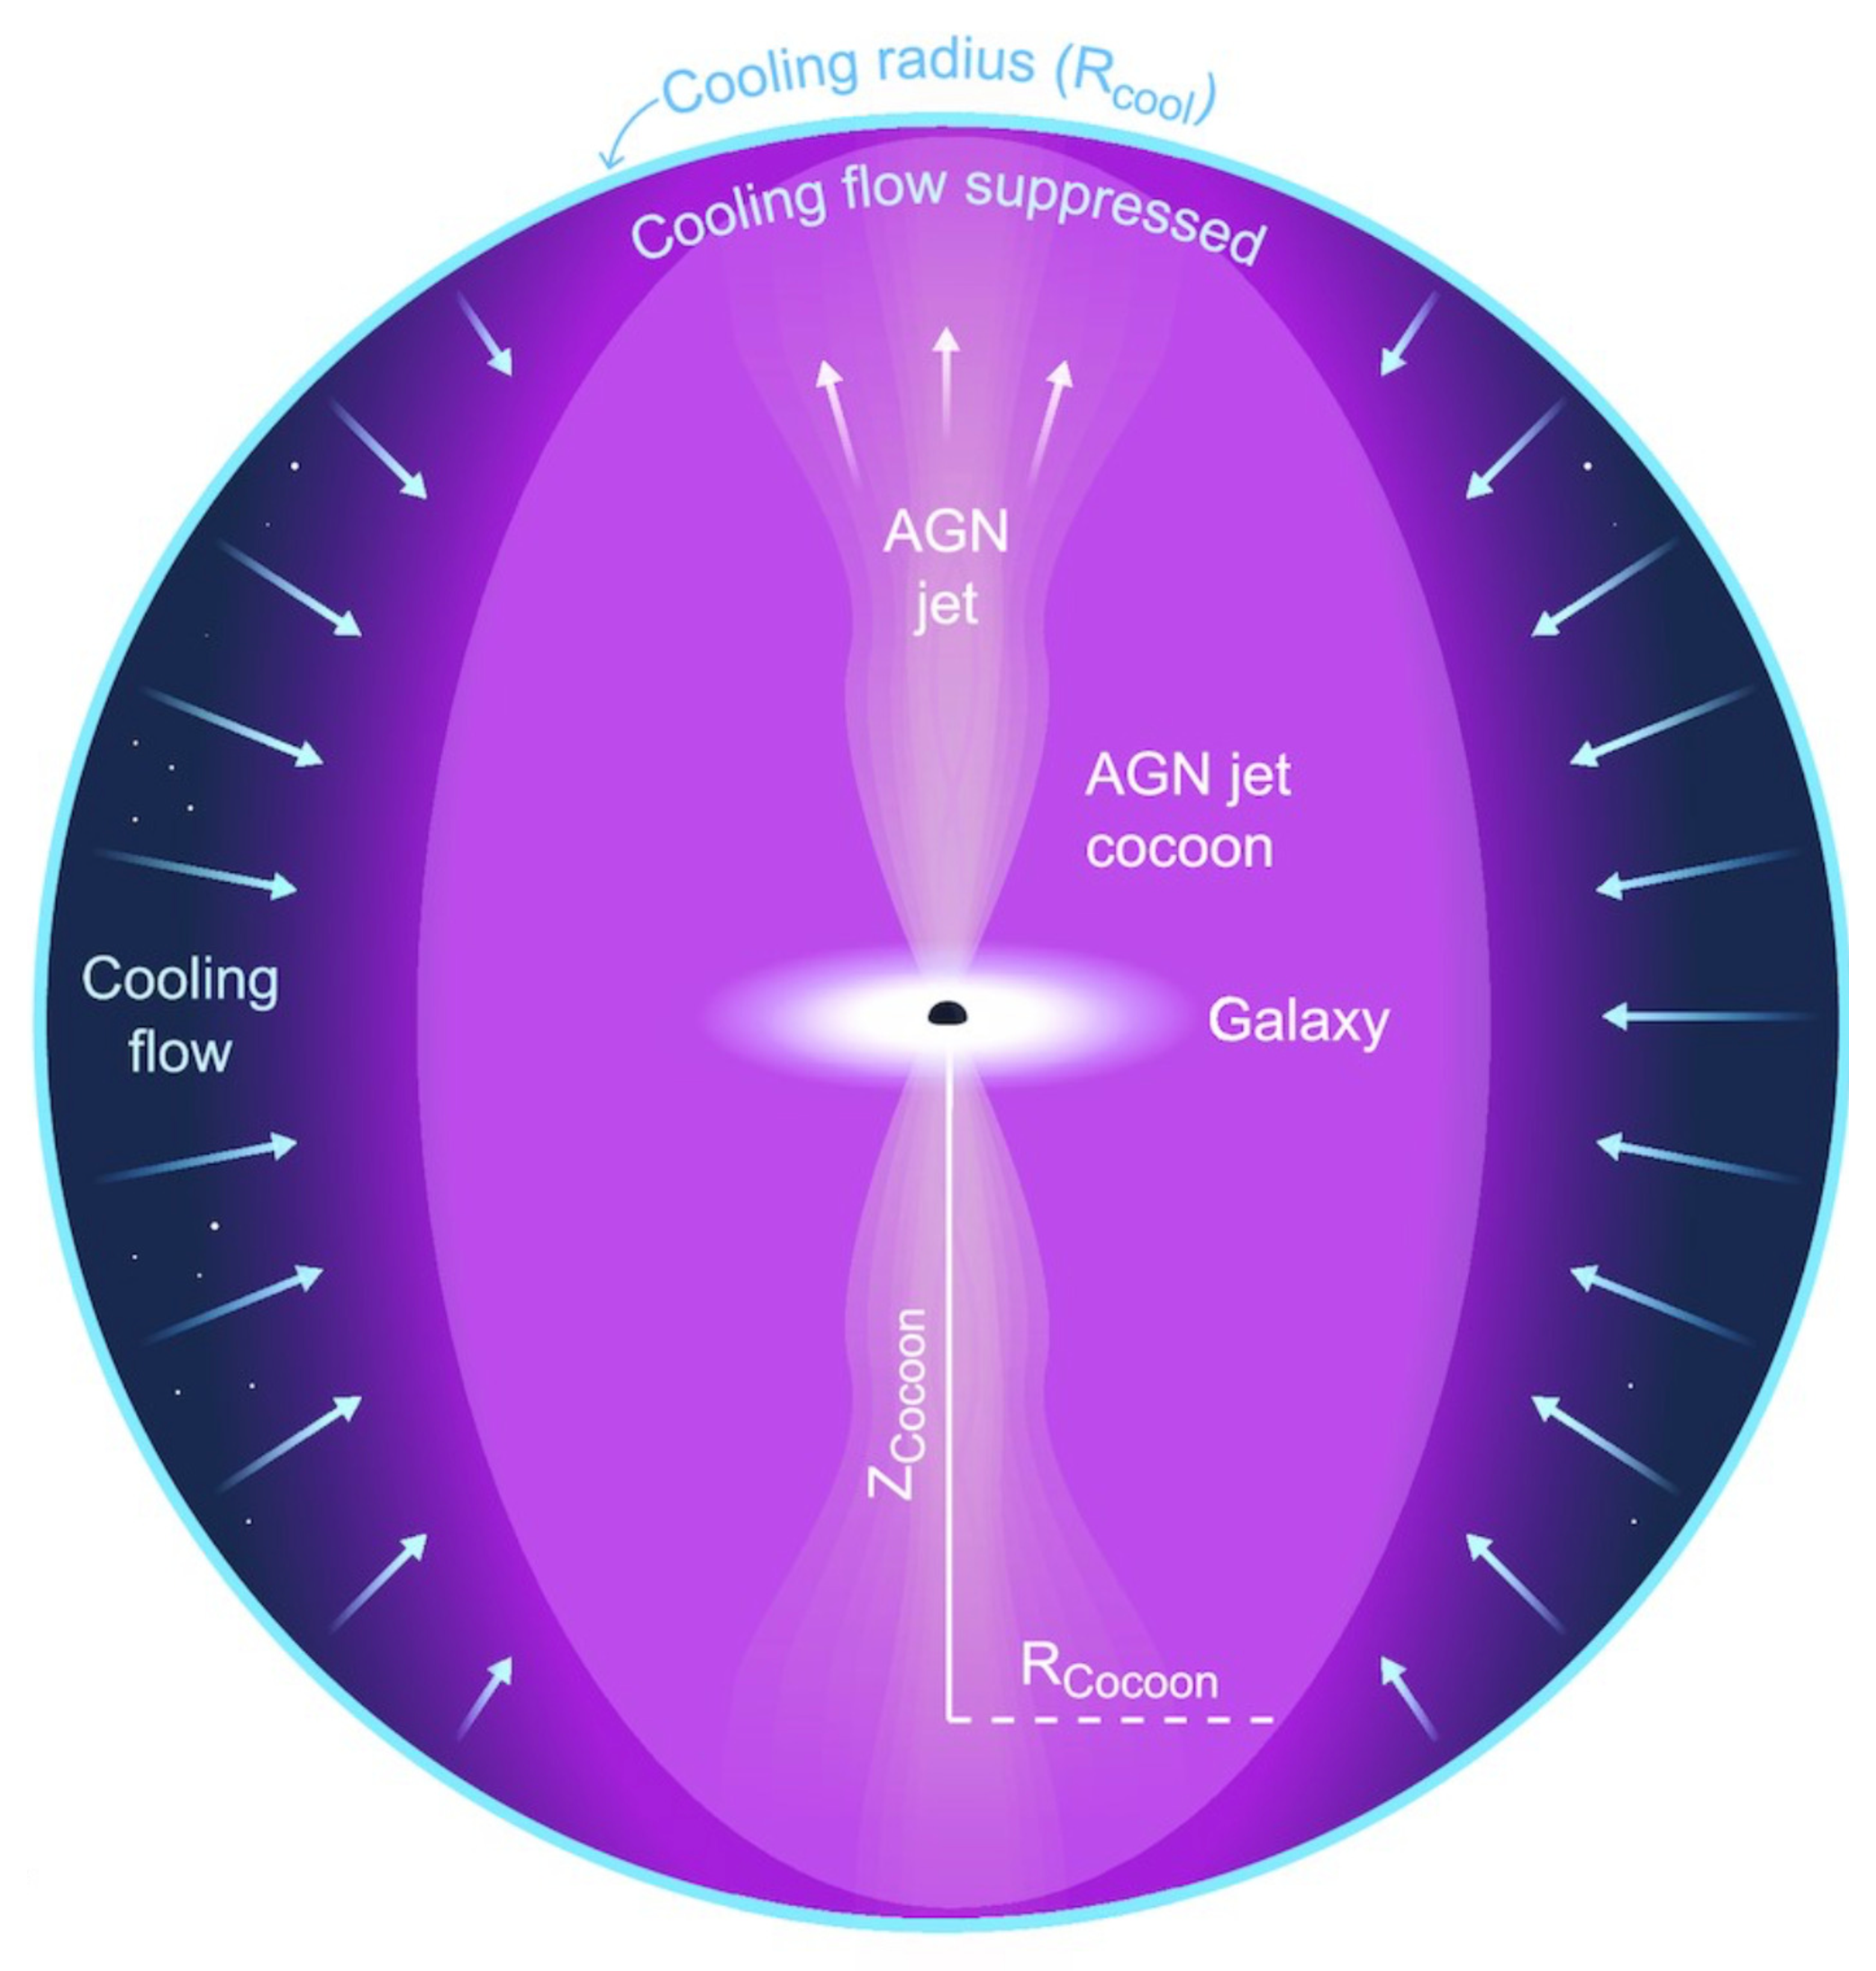
\includegraphics[width=0.8\linewidth]{Sim_img/AGN-cycle.pdf}
    \caption{Adapted from Figure 7 of \citet{su_which_2021}; illustration of the feeding-feedback cycle in AGNs. Jet feedback drives turbulence in the circumgalactic medium (CGM) and facilitates gas mixing, which heats the galaxy at kpc scales. The mixture of warm gas continues to cool and cascade toward the plane of the galaxy. The gas ends up in an accretion disk perpendicular to the jet direction, and a fraction of it is accreted, while the rest interacts with the central engine and is launched outward via AGN jets, repeating the cycle.}
    \label{fig:multiscale-accretion}
\end{figure}

Many galaxy clusters harbor extended radio emission from the central AGN jet.
For example, the Virgo cluster (which hosts the galaxy M87 at its center) and the Centaurus cluster both have radio jets extending beyond $\sim 10$\,kpc from the cluster core.
Others, like Perseus, are known for X-ray cavities in the ICM, which are thought to be inflated by AGN jets and then rise away from the cluster core \citep{fabian_chandra_2000}.
The hot and energetic jet material collides with the surrounding medium and drives turbulence in the ICM, providing further kinetic pressure support against a cooling flow \citep{hitomi_collaboration_atmospheric_2018}.
These observations identify AGN jets as the likely source of heating, but leave open how jet energy is deposited into the gas and transported across scales to the galaxy core.

Because AGN jet power ultimately depends on gas accretion onto the central SMBH, the accretion flow is inextricably linked to the jet feedback that suppresses the cooling flow.
During periods of weak feedback, pressure support decreases, leading to a higher cooling rate and more accretion.
This large amount of matter accumulates in the accretion disk, extracting more energy from the black hole, which begins a period of strong jet feedback.
As the AGN jet pushes outward and collides with the surrounding medium, it heats up the galaxy, effectively shutting down cooling.
Without cooling, accretion is quenched, and the black hole goes into a quiescent phase, starting the cycle again.
Figure~\ref{fig:multiscale-accretion} shows an illustration, adapted from Fig.~7 of \citet[][]{su_which_2021}, of the feeding-feedback cycle in AGNs.

\subsection{The gap in our theoretical understanding of meso-scale accretion flows and their connection to AGN feeding and feedback}

AGN feedback depends strongly on the accretion state of the central SMBH\@.
Low-luminosity AGNs (LLAGNs), such as M87$^{\star}$ and Sagittarius A$^{\star}$, accrete matter at much lower rates than the theoretical Eddington limit ($\dot{M}_{\rm BH} \ll \dot{M}_{\rm Edd}$), while quasars accrete matter rapidly ($\dot{M}_{\rm BH} \sim \dot{M}_{\rm Edd}$).
At low accretion rates, feedback is mainly provided by the SMBH-driven jet---the \textit{radio-mode feedback}; at high accretion rates, feedback is more complex, but often dominated by radiation-driven pressure from the large amount of matter being actively accreted \citep[e.g.,][]{cielo_agn_2018}---the \textit{quasar-mode feedback}.

This chapter focuses on radio-mode feedback and the regulation of quiescent elliptical galaxies by AGN jets, with M87 as the central example.
M87 is the central galaxy of the Virgo cluster and hosts a SMBH \citep[$M_{\rm BH} \approx 6.5\times10^9\, M_{\odot}$;][]{eht_one}.
Because X-ray observations of AGNs struggle to probe the region near the SMBH \citep[e.g.,][]{snios_detection_2019}, $\dot{M}_{\rm BH}$ is often estimated using the Bondi accretion model \citep[][]{bondi_spherically_1952}.
For M87, however, estimates of \mdotbh\ from AGN luminosity and EHT observations are several orders of magnitude below the Bondi estimate \citep[][]{russell_radiative_2013,eht_eight}.
Follow-up X-ray observations also show that the density and temperature profiles inside the Bondi radius of M87 do not agree with the predicted profiles of Bondi accretion \citep[e.g.,][]{russell_inside_2015}.
In addition, M87 hosts multiphase gas with an additional $T \sim 10^4\,K$\ component, including gas observed in a disky structure \citep[e.g.,][]{walsh_m87_2013,lu_ring-like_2023}.
These discrepancies suggest that Bondi accretion is not the correct assumption for M87 or many other LLAGNs.

Despite evidence against the Bondi model, many state-of-the-art cosmological simulations still employ this framework to approximate the amount of feedback produced by galaxies \citep[e.g.,][]{dave_simba_2019,pakmor_millenniumtng_2023}.
At the opposite end of the spatial scale, general relativistic magnetohydrodynamic (GRMHD) simulations have successfully revealed the complex dynamics of the accretion flows near the event horizon, and their results generally agree with recent EHT observations of the accretion flows onto M87$^{\star}$ and Sagittarius A$^{\star}$ \citep{eht_one,eht_sgt_one}.
These simulations, however, are often initialized with a simple idealized torus inside a toroidal magnetic field \citep[e.g.,][]{white_structure_2020,kaaz_nozzle_2023}.
Such initial conditions are simple to set up, but lack physical motivation, and the results have been shown to be sensitive to the exact starting conditions \citep[see][]{davis_magnetohydrodynamics_2020}.
The work presented in this chapter addresses the gap between observations and simulations by studying multiphase accretion flows through eight orders of magnitude in scale.
By reaching the inner accretion disk region of the SMBH, it also provides physically motivated initial and boundary conditions for future GRMHD simulations, whose results can then be directly compared to observations made by the EHT\@.
Figure~\ref{fig:theory-gap} summarizes the field's need for this connection between resolved simulations and observations.

\begin{figure}
    \centering
    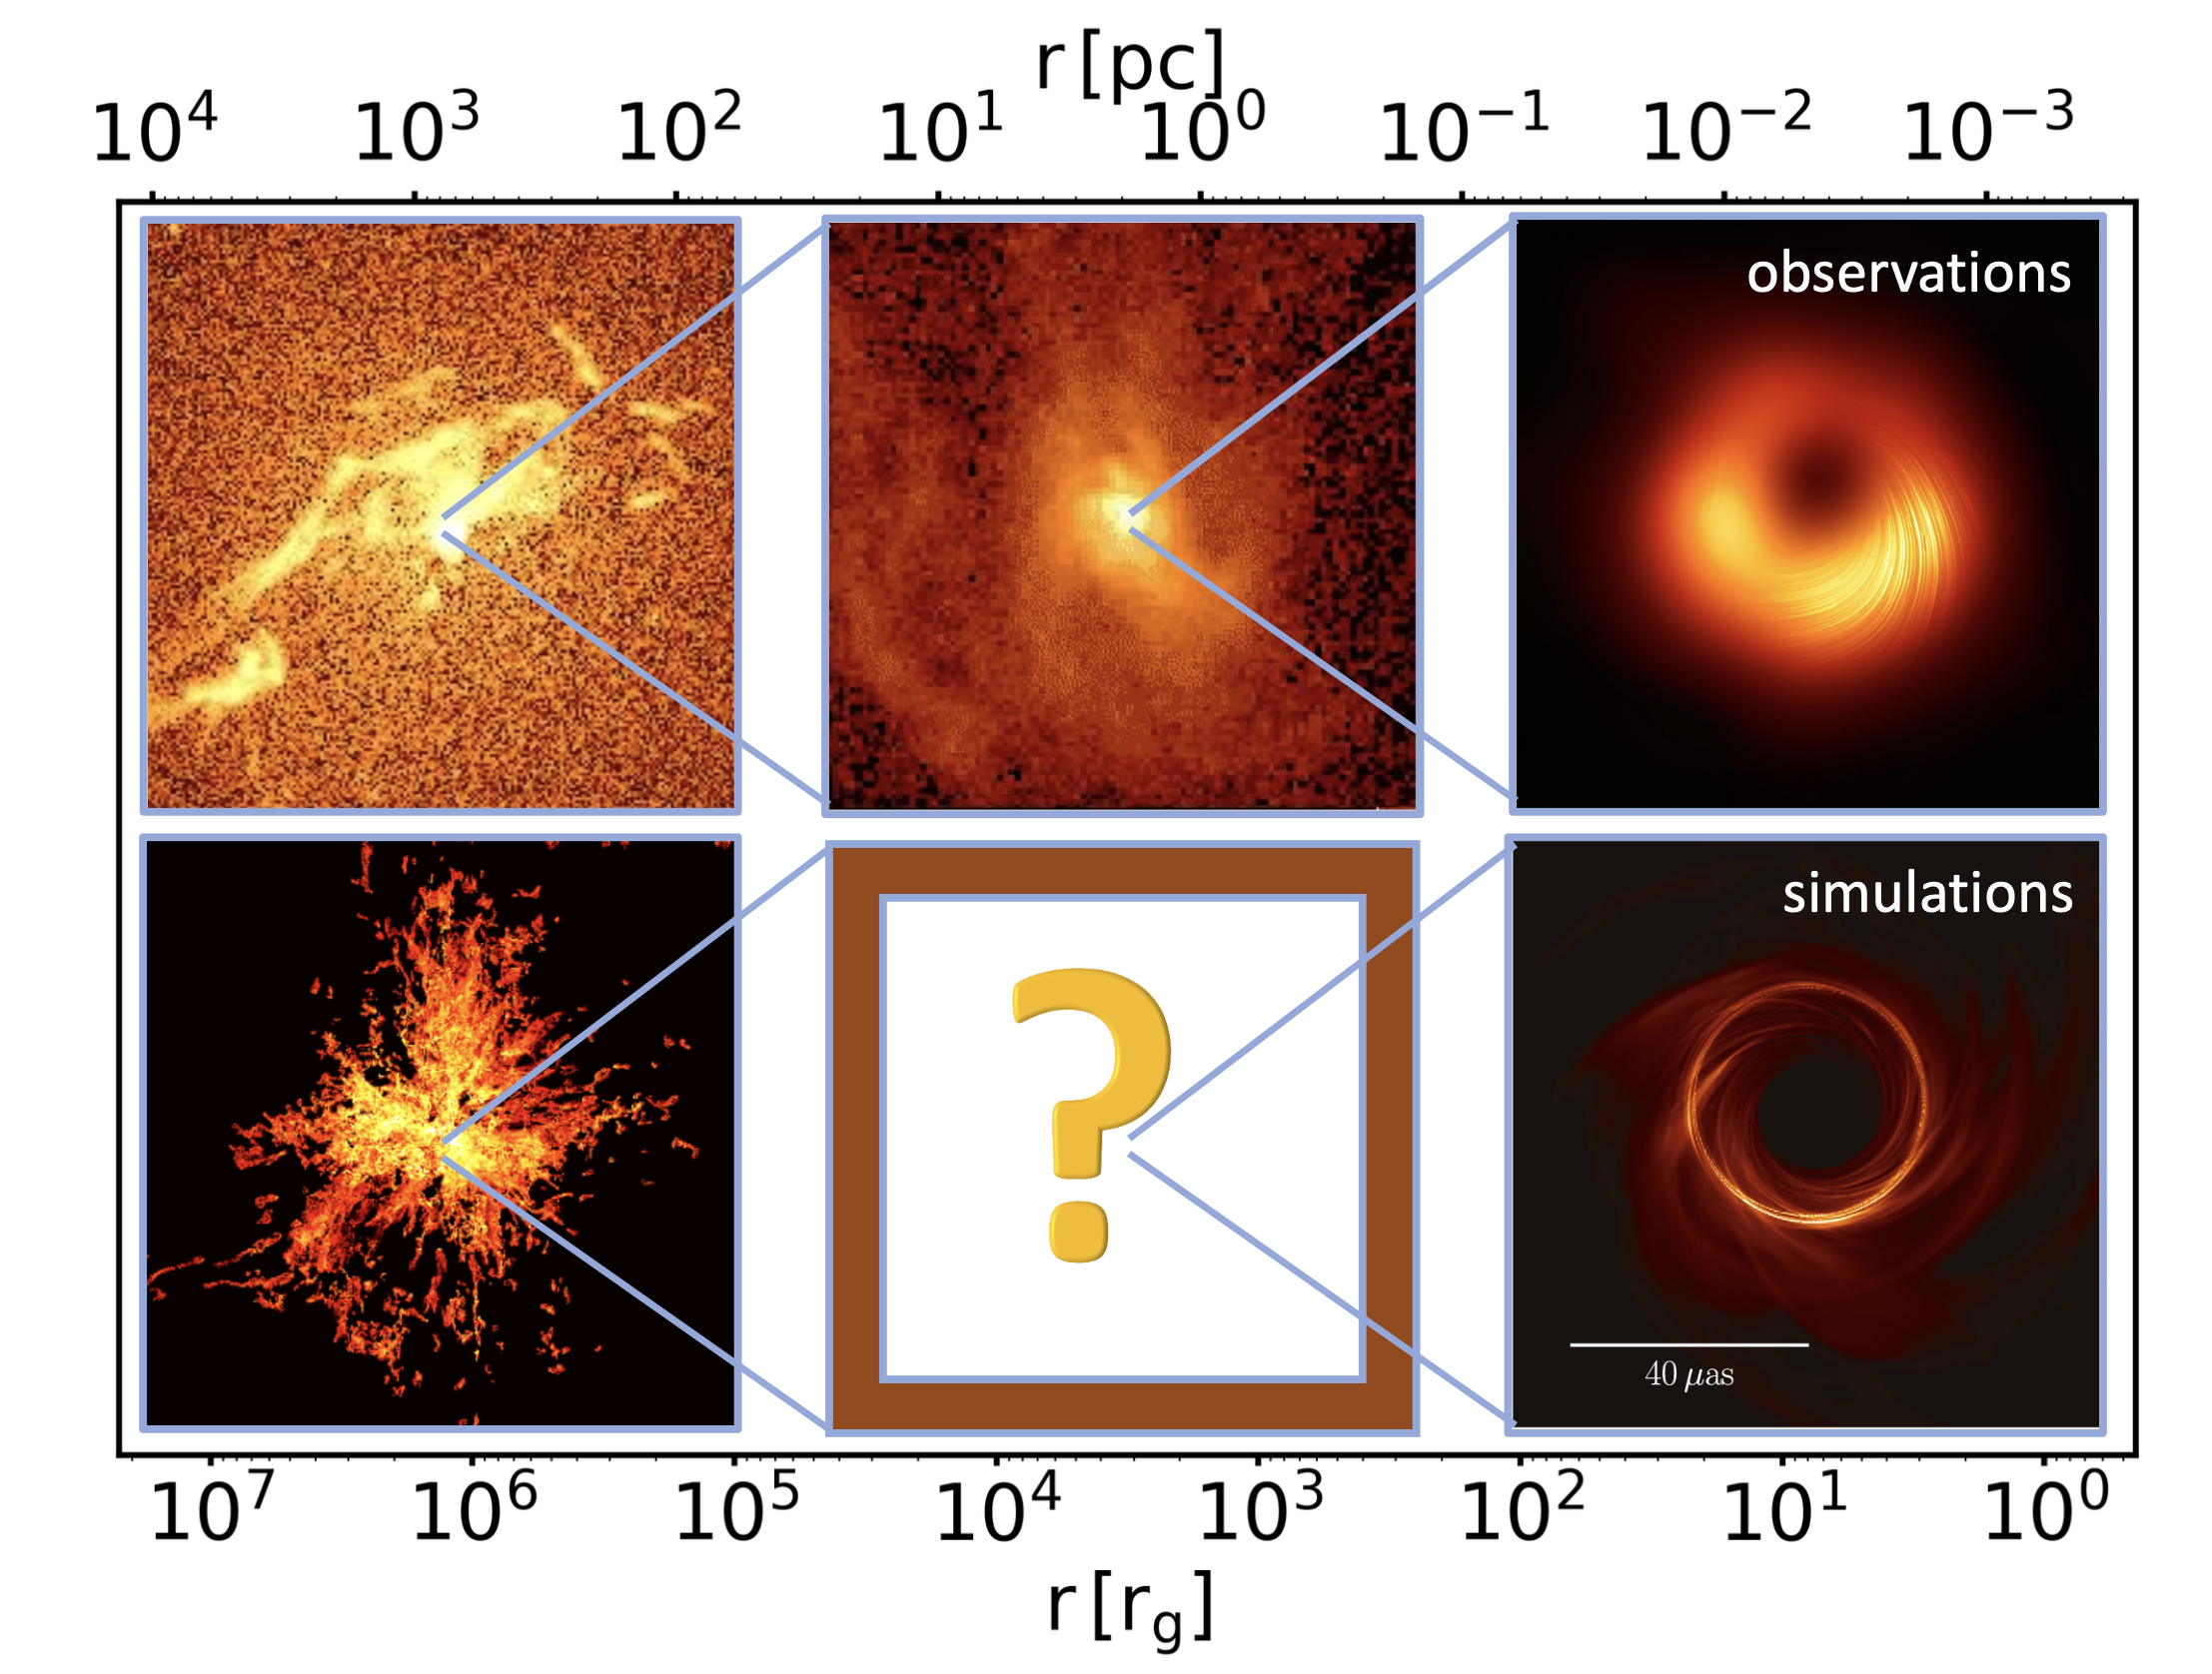
\includegraphics[width=0.8\linewidth]{Sim_img/gap_theory.png}
    \caption{
    Observations of M87 (top panels) from galaxy scale to event-horizon scale (left to right) compared with numerical simulations (bottom panels).
    Top left panel: (MUSE) \halpha+[\ion{N}{2}] image of the central $\sim 10$\,kpc region of M87 \citep{boselli_virgo_2019}.
    Top middle panel: (Hubble) \halpha\ image of the central few hundred pc of M87 \citep{walsh_m87_2013}.
    Top right panel: EHT image of the accretion flow near the SMBH in the center of M87 \citep{eht_one}.
    Bottom left panel: \halpha\ map of the central tens of kpc of a simulated cluster central galaxy \citep{li_cooling_2015}.
    Bottom right panel: GRMHD simulation of the M87 SMBH \citep{eht_one}.
    On the meso-scale, from the Bondi radius (hundreds of pc) to the outer edge of the accretion disk, the observed accretion flow is multiphase and dynamically complex, but theoretical understanding lags behind observations. This chapter addresses this gap and bridges two important scales in SMBH accretion studies. Credit: Yuan Li.}
    \label{fig:theory-gap}
\end{figure}

The following section is adapted from Ha \& Li 2026, manuscript in preparation.

\section{Gas Morphology and Accretion Dynamics of Multiphase Accretion onto SMBHs}

\publicationdetails[From]
{Ha \& Li 2026, manuscript in preparation}
{Trung Ha\footnotemark[1] and Yuan Li\footnotemark[1]}
{Low-luminosity active galactic nuclei regulate the hot atmospheres of massive elliptical galaxies through jet-driven feedback, yet the accretion flow linking kpc-scale cooling to event-horizon-scale black hole feeding remains poorly understood. We study multiphase, multi-scale accretion in elliptical galaxies with a suite of hydrodynamic (HD) simulations. We initialize the galaxy using profiles motivated by \textit{Chandra} observations of M87 and the Virgo cluster, and use nested static mesh refinement (SMR) to follow the gas from the kpc scale down to $\sim 50\,r_{\rm g} \approx 16$\,mpc. We find that AGN jet feedback facilitates the formation of cool gas filaments at the kpc scale. These filaments carry angular momentum and circularize into a disk as the accretion flow is resolved to smaller radii. Outside $\sim 10^3\,r_{\rm g}$, the hot and cool phases are dynamically decoupled: the cool gas primarily forms rotationally supported disks, while the hot gas accretes more radially. Inside this scale, the cool gas is compression-heated to the virial temperature, and the innermost accretion flow becomes dominated by the hot phase. The net inflow rate follows a radial scaling $\dot{M}\propto r^k$, with $0.40 \leq k \leq 0.69$, broadly consistent with previous results for radiatively inefficient accretion flows (RIAFs). We also revisit the Bondi accretion model in this multiphase environment. We find that the Bondi model can estimate the hot gas inflow rate, but does not describe the cool, rotationally supported accretion flow. Our results suggest that unresolved black hole accretion rates in galaxy-scale and cosmological simulations should be estimated from the hot gas inflow outside the cool gas precipitation radius, then scaled inward using the measured accretion-rate relation.}
{\footnotetext[1]{Department of Astronomy, University of Massachusetts Amherst, Amherst, MA 01003, USA}}
\setcounter{footnote}{0}

\subsection{Introduction}
\label{sec:agn-intro}

The centers of most galaxies host supermassive black holes \citep[SMBHs,][]{magorrian_demography_1998,kormendy_coevolution_2013}.
When SMBHs accrete at high rates ($\dot{M} \gtrsim 10^{-3} \dot{M}_{\rm Edd}$, where $\dot{M}_{\rm Edd}$\ is the Eddington accretion rate), their accretion disks are radiatively efficient, and feedback is dominated by radiation pressure associated with the large inflow of matter \citep[e.g.,][]{cielo_agn_2018}. This regime is commonly referred to as \textit{quasar-mode feedback}.
Quasar-mode feedback is important in high-redshift active galactic nuclei \citep[AGNs, e.g.,][]{di_matteo_energy_2005}, but is less commonly seen in the local universe.
At low accretion rates ($\dot{M} \ll \dot{M}_{\rm Edd}$), the accretion disks are radiatively inefficient. Feedback is predominantly mechanical, mediated by relativistic jets that produce radio emission. The regime is thus known as \textit{radio-mode feedback} \citep[][]{mcnamara_heating_2005}.
These systems are typically observed as low-luminosity AGNs and constitute $\approx 99\%$ of the AGN population in the local universe \citep[][]{birchall_incidence_2022}.


Current theory and observations support a picture in which SMBH jet-driven feedback regulates the atmosphere of the host galaxies of low-luminosity AGNs \citep[][]{mcnamara_mechanical_2012}.
In this picture, jets inject energy into the surrounding medium, which suppresses cooling and star formation \citep[][]{combes_agn_2017}.
As cooling slows down, the fuel supply diminishes, jet power declines, and cooling can resume, repeating the cycle.
Many systems, such as M87 and other central galaxies in galaxy clusters and groups, are observed to harbor spatially extended cool clouds \citep[e.g.,][]{edge_detection_2001,salome_cold_2003,simionescu_alma_2018,boselli_virgo_2019}. These cool clouds often appear filamentary on kpc to tens of kpc scales, and exhibit a lack of large-scale coherent motion \citep[e.g.,][]{olivares_ubiquitous_2019}. Numerical simulations show that the cool clouds may have condensed out of the hot atmosphere due to thermal instability \citep{mccourt_thermal_2012,sharma_thermal_2012}, which can be triggered by jet feedback \citep{li_2014a}. The fate of the multiphase gas is unclear. While some observations suggest that the cool clouds may be directly feeding the SMBH as cold clumps \citep[e.g.,][]{tremblay_cold_2016}, recent high-resolution observations suggest that the multiphase gas may settle into a rotating structure at the $\sim100$\,pc scale \citep{osorno_revisiting_2023,oosterloo_closing_2023,tamhane_hst_2026}.


Two main uncertainties in understanding radio-mode SMBH feeding and feedback are the mass accretion rate onto SMBHs, \mdotbh, and the phase of the accretion flow. \mdotbh\ is difficult to measure directly because of the extremely high resolution required.
One common way to estimate the accretion rate is using the classical Bondi-Hoyle-Lyttleton model \citep[hereafter the ``Bondi model'',][]{hoyle_effect_1939,bondi_mechanism_1944,bondi_spherically_1952}.

For M87, gas properties measured near $r_{\rm B}\approx120$\,pc (five orders of magnitude larger than the event horizon of the SMBH) imply a Bondi accretion rate of $\dot{M}_{\rm B} \approx 0.1\, M_{\odot}\, \mathrm{yr}^{-1}$ \citep[][]{di_matteo_accretion_2003, russell_inside_2015}.
However, estimates of \mdotbh\ via other methods, such as AGN luminosity \citep[][]{broderick_event_2015}, Faraday rotation \citep[][]{kuo_measuring_2014}, and Event Horizon Telescope \citep[EHT,][]{eht_eight} observations are at odds with the Bondi estimate, often orders of magnitude smaller than \mdotb.
This discrepancy suggests that the Bondi model's assumptions of spherical accretion and a homogeneous, single-phase medium do not capture the multiphase, turbulent, and rotating accretion flows expected around low-luminosity AGNs.

Despite the Bondi model's overestimation of the true accretion rates in low-luminosity AGNs, many state-of-the-art cosmological simulations still adopt this model or close variants to estimate \mdotbh\ and the associated feedback power \citep[e.g.,][]{schaye_eagle_2015, tremmel_romulus_2017,pillepich_simulating_2018,dave_simba_2019,pakmor_millenniumtng_2023}.
This is largely because their typical resolutions ($\sim 0.1$--$1$\,kpc) cannot resolve the relevant black hole accretion physics.

A multi-scale numerical study that connects the gas at the galaxy-scale to the accretion flow at the event-horizon-scale is needed to provide better subgrid prescriptions of SMBH accretion in cosmological simulations.
Recent efforts have pursued this goal using a range of strategies, including hyper-refinement of selected halos from cosmological simulations \citep[e.g.,][]{angles-alcazar_cosmological_2021,hopkins_forged_2024,kaaz_h-amr_2025}, repeated zoom-ins of individual galaxies \citep[e.g.,][]{ressler_ab_2020,guo_toward_2023,guo_magnetized_2024}, reduced scale separation \citep[e.g.,][]{lalakos_bridging_2022}, and multi-zone or cyclic approaches spanning many length scales \citep[e.g.,][]{yuan_numerical_2012,cho_multizone_2024,guo_cyclic_2025}.

In this work, we study the formation and dynamics of a multiphase accretion flow under the influence of jet feedback in an idealized galaxy based on the nearby radio galaxy M87, the central galaxy of the Virgo cluster.
M87 hosts a SMBH of mass $M_{\rm BH} \approx 6.5\times10^9\,\mathrm{M_{\odot}}$ \citep[][]{eht_six} and has been the focus of extensive multiwavelength observations.
On kiloparsec scales, extended multiphase filaments are observed \citep{boselli_virgo_2019}. On tens-of-parsec scales, a multiphase circumnuclear disk has also been observed \citep{walsh_m87_2013}.
On horizon scales, the EHT has imaged the shadow of M87$^{\star}$ \citep[][]{eht_one}, and recent observations have begun to directly link the inner accretion flow to the emerging jet \citep[][]{lu_ring-like_2023}.
Together, these observations make M87 a prime candidate for testing models of multiphase feeding and jet feedback across vast spatial scales.



Using a suite of hydrodynamic (HD) simulations spanning from galaxy scales to tens of Schwarzschild radii, we study the rate, phase, morphology, and kinematics of the accretion flow.
The paper is organized as follows. In Section~\ref{sec:method}, we describe the numerical methods and physical models used in the galaxy-scale and meso-scale simulations. In Section~\ref{sec:galaxy-scale-result}, we present the galaxy evolution over 2\,Gyr. We discuss the multi-scale accretion dynamics, disk formation, and thermodynamics in Section~\ref{sec:zoom-in-result}. We discuss the Bondi accretion model in the context of a turbulent, multiphase environment, the effects of the size of the accretion zone on the cool phase's filamentary, chaotic accretion, as well as limitations of our simulations in Section~\ref{sec:discussion}. We conclude and summarize our main results in Section~\ref{sec:conclusion}.





\subsection{Methodology} \label{sec:method}

\begin{table}
\centering
\caption{Initial conditions\label{tab:initial-condition}}
\begin{tabular}{lcc}
\hline
\hline
Parameter & Value & Equation \\
\hline
Physical parameters & & \\
$K_0$ & 7 keV\,cm$^2$ & \ref{eq:entropy} \\
$\Gamma$ & 1.1 & \ref{eq:entropy}\\
$x$ & $r/(2\,\rm kpc)$ & \ref{eq:entropy} \\
$n (x=1)$ & 0.1 cm$^{-3}$ & \ref{eq:pressure} \\
$M_{\rm BH}$ & $6.5 \times 10^9 M_{\odot}$ & \ref{eq:gacc} \\
$M_{\rm DM}$ & $3 \times 10^{13} M_{\odot}$ & \ref{eq:gacc} \\
$R_{\rm DM}$ & $60$\,kpc & \ref{eq:gacc}\\
$M_{\star}$ & $3 \times 10^{11} M_{\odot}$ & \ref{eq:gacc} \\
$R_{\star}$ & $2$\,kpc & \ref{eq:gacc} \\
\hline
Simulation parameters & & \\
$L_{\rm box}$ & 128 kpc & \\
$R_{\rm out}$ & 64 kpc & \\
$n (r<R_{\rm acc})$ & $5 \times 10^{-3}$\,cm$^{-3}$ & \\
$T_{\rm floor}$ & $2\times10^5$\,K & \\
$n_{\rm floor}$ & $10^{-3}$\,cm$^{-3}$ & \\
$v_{\rm jet}$ & 3000 km\,s$^{-1}$ & \ref{eq:jet-momentum} \\
\hline
\end{tabular}
\parbox{0.6\linewidth}{\footnotesize \textit{Note.} The ``Equation'' column denotes the first instance in which the parameter is referenced.}
\end{table}



We carry out three-dimensional (3D) HD simulations using the \ath\ code \citep{stone_athena_2020}.
\ath~is a grid-based numerical code for astrophysical fluid dynamics simulations.

We solve the hydrodynamic equations using the Harten--Lax--van Leer--Contact Riemann solver, a piecewise linear reconstruction method, and a second-order Runge-Kutta time integrator.


Overall, the code solves the following HD equations:
\begin{equation}
    \frac{\partial \rho}{\partial t} + \nabla \cdot (\rho \mathbf{v}) = 0,
\end{equation}
\begin{equation}
    \frac{\partial \rho \mathbf{v}}{\partial t} + \nabla \cdot (P \mathbf{I} + \rho \mathbf{v} \mathbf{v}) = \rho \mathbf{g},
\end{equation}
\begin{equation}
    \frac{\partial E}{\partial t} + \nabla \cdot [(E+P)\mathbf{v}] = \rho \mathbf{g} \cdot \mathbf{v} - Q_{-},
\end{equation}
which are the continuity equation, the momentum conservation equation, and the energy conservation equation, respectively.
$Q_{-}$\ is the heat loss per unit volume due to radiative cooling.
We do not include any explicit heating term in our simulations, but heat can be generated through numerical dissipation of shocks and turbulence.


\subsubsection{Initial conditions} \label{subsec:init}

Our galaxy-scale simulations use a hydrostatic equilibrium initial condition based on the observations of the Virgo cluster \citep{urban_x-ray_2011} and of its central galaxy M87 \citep{russell_inside_2015}.
We start with a flat core entropy profile following \citet{martizzi_simulations_2019}:
\begin{equation}
\label{eq:entropy}
    K_{\rm gas}(x) = \frac{K_0}{2}(1+x^{\Gamma}),
\end{equation}
where $K_{0}=7$~keV cm$^2$, $\Gamma = 1.1$, and $x \equiv r/(2~\mathrm{kpc})$~is the dimensionless length scale of the system \citep{urban_x-ray_2011}.
The pressure is a function of the entropy and the gas number density:
\begin{equation}
\label{eq:pressure}
    P(x) = K_{\rm gas}(x) \cdot n(x)^{\gamma},
\end{equation}
where $\gamma = 5/3$ is the adiabatic gas index.

Assuming hydrostatic equilibrium:
\begin{equation}
    \frac{dP(r)}{dr} + \rho g = 0\, ,
\end{equation}
we have
\begin{equation}
\label{eq:dn_dx}
    \frac{dn}{dx} = \frac{2 (r_0 / K_0) \mu m_{\rm H} n(x)^{2-\gamma} \cdot g - \Gamma n(x) \cdot x^{\Gamma - 1} }{1+x^{\Gamma}\gamma},
\end{equation}
where $n$ is the number density, $\mu \approx 0.6$\ is the mean molecular weight, and $m_{\rm H}$\ is the hydrogen mass.
Using the observed density $n(x=1)=0.1\,\mathrm{cm}^{-3}$ \citep{russell_inside_2015}, we numerically solve Equation~\ref{eq:dn_dx} for $n(x)$ using a fourth-order Runge-Kutta scheme.
At time $t= 0$, we verify that the density and temperature profiles closely match the observed profiles (see Figure~\ref{fig:r-prof-meso}).

We inject a small density perturbation on the order of a few percent ($\sim 5\%$) on top of the hydrostatic equilibrium solution, using a Gaussian noise distribution, to seed initial instability.
A summary of the physical parameters, as well as the global simulation parameters, is listed in Table~\ref{tab:initial-condition}.

\begin{table}
\centering
\caption{Simulations and parameters\label{tab:simulations}}
\begin{tabular}{lccccc}
\hline
\hline
Name & \racc\ (mpc) [($r_{\rm g}$)] & $N_{\rm refine}$ & $t_{\rm start}$ (Myr) & $\Delta t$ (Myr) \\
(1) & (2) & (3) & (4) & (5) \\
\hline
Galaxy-scale \\
R8 & $4^8$ [$2.1 \times 10^5$] & 8 & 0 & 2000 \\
\hline
Zoom-in \\
R10 & $4^7$ [$5.3 \times 10^4$] & 10 & 920 & 50 \\
R12 & $4^6$ [$1.3 \times 10^4$] & 12 & 925 & 5 \\
R14 & $4^5$ [$3.3 \times 10^3$] & 14 & 928 & 2 \\
R16 & $4^4$ [$8.2 \times 10^2$] & 16 & 929.25 & 0.5 \\
R18 & $4^3$ [$2.1 \times 10^2$] & 18 & 929.55 & 0.05 \\
\hline
Meso-scale \\
R20 & $4^2$ [$5.1 \times 10^1$] & 20 & 929.57 & 0.003 \\
\hline
\end{tabular}

\vspace{0.5em}
\parbox{0.75\columnwidth}{\small\textit{Note.} The galaxy-scale simulation is run first, then snapshots of interest are selected for resimulation with additional nested refinement. The columns list, from left to right: (1) name of the simulation, (2) radius of the accretion zone, (3) number of nested refinement levels, (4) start time of the simulation, (5) duration of the simulation.}
\end{table}


\subsubsection{Galaxy-scale simulation setup} \label{subsec:setup}

Our simulations use Cartesian grids.
The root grid consists of $128^3$ cells with a domain width of $L_{\rm box} = 128$\,kpc.
This translates to a root resolution of $\Delta x_{\rm max} = 1$\,kpc.
At each refinement level $\ell$, the center 64 cells per dimension of level $\ell-1$\ are replaced by twice as many cells with half the width, reaching a spatial resolution of  $\Delta x_{\rm min} = 1/2^{\ell}$\,kpc.
We apply 8 levels of nested static mesh refinement (SMR) to our galaxy-scale simulation, which allows us to resolve the accretion flows down to $\Delta x_{\rm min,R8}\approx 4$\,pc at the center of the domain.

We perform several galaxy-scale simulations with varying jet parameters, such as the jet kinetic fraction ($f_{\rm kin}$), the height and width of the jet base (see Section~\ref{subsubsec:jet}). Each is evolved for 1 Gyr, except for the fiducial run which is evolved for 2 Gyr.
We mainly focus on the results from the fiducial run, R8, in this paper.

A spherically symmetric outer boundary condition is implemented at $R_{\rm out} = 64$\,kpc, where primitive variables ($\rho,\ p,\ \mathbf{v}$) are reset to an initial hydrostatic equilibrium solution at each time step.
An inner boundary of a spherical accretion (sink) region is set up near the center of the domain at $R_{\rm acc,R8} = 4^8\,\mathrm{mpc}\approx 65.5$\,pc initially. We gradually shrink this boundary for the meso-scale simulations, described in \fullsectionref{subsec:meso}.
This region acts like a ``vacuum'' zone, where the density is reset at every step to $n_{r < R_{\rm acc}} = 5\times 10^{-3}~\mathrm{cm^{-3}}$ and the temperature is reset to the global floor temperature $T_{r < R_{\rm acc}} = T_{\rm floor}$.
This inner boundary accretion region can prevent unrealistic pressure bounces as gas builds up in the center of the domain, following a numerical treatment similar to \citet{guo_toward_2023}. We also track the accretion rate through this boundary as a proxy for the black hole accretion rate.

The galaxy-scale simulations include several physical processes important in regulating the feeding--feedback balance in M87: static gravitational potential, radiative cooling, and AGN jet feedback.
Below, we discuss our implementation of each process in more detail.

\centerline{\textbf{Static gravitational potential}} \label{subsubsec:grav}


We model the SMBH as a point mass with $M_{\rm BH} = 6.5 \times 10^9~M_{\odot}$ \citep[e.g.,][]{eht_six}, and we model both the dark matter halo and the stars as Navarro-Frenk-White (NFW) profiles \citep{navarro_structure_1996}.
The mass enclosed at a given distance $r$ from the SMBH is:
\begin{equation}
\label{eq:mass}
    M(r) = M_0 \left[\ln(1 + \frac{r}{r_0}) - \frac{r}{r + r_0}\right],
\end{equation}
where $M_0 = 3\times10^{13} M_{\odot}$ and $r_0 = 60$~kpc for the dark matter halo, and $M_0 = 3\times10^{11} M_{\odot}$ and $r_0 = 2$~kpc for the stars.
These parameters are chosen such that the mass profiles match the observed profiles in \citet{gebhardt_black_2009}.

The gravitational acceleration as a function of distance from the SMBH is then:
\begin{equation}
\label{eq:gacc}
    \mathbf{g}(r) = - \frac{G(M_{\rm BH} + M_{\rm DM}(r) + M_{\star}(r))}{r^2} \hat{\mathbf{r}}.
\end{equation}
Inside the accretion zone, we multiply $\mathbf{g}(r)$\ by a softening factor, $F_s$, to prevent fast-moving accreted gas from escaping the sink before it is removed,
following \citet{guo_toward_2023}:
\begin{equation}
    F_s|_{r < R_{\rm acc}} = \frac{r^3 (1-e^{-r^{2}/r_{a}^2})}{(r^2 + r_{a}^2 \cdot e^{-r^{2}/r_{a}^2})^{3/2}},
\end{equation}
where $r_{a} = R_{\rm acc}/2$.

\centerline{\textbf{Radiative cooling}}

We model radiative cooling as a source term in the simulation:
\begin{equation}
    Q_{-} = n^2\Lambda(T),
\end{equation}
where $n$ is the number density in cm$^{-3}$, and $\Lambda(T)$ is the cooling function in erg s$^{-1}$~cm$^3$, modeled as a piecewise function of the temperature, assuming solar metallicity.

At $\log T > 8.15$,
\begin{equation}
    \Lambda(T) = 10^{-26.065}T^{0.45},
\end{equation}
following \citet{schneider_introducing_2018}.
For $\log T \leq 8.15$, we interpolate to obtain $\Lambda(T)$~from a tabulated emissivity curve following Table 2 of \citet{schure_new_2009}.

In most of our simulations, we force a temperature floor at $T_{\rm floor}=2\times10^5$\,K, but in several short-term runs, we set the temperature floor to $10^4$\,K (see Section~\ref{subsec:limitations}).
A global number density floor is also applied at $n_{\rm floor} =10^{-3}\,\mathrm{cm^{-3}}$.
Throughout this paper, we refer to gas at temperatures below and above $10^6$\,K as the cool and hot phases, respectively.

\centerline{\textbf{Black hole accretion and AGN jet feedback}}
\label{subsubsec:jet}

We compute the black hole accretion rate by measuring the accretion rate at the inner boundary of the simulation, then scaling the value as follows:
\begin{equation}
\label{eq:scaling}
    \dot{M}_{\rm BH} = \dot{M}_{|R_{\rm acc}} \cdot \left(\frac{100\,r_{\rm g}}{R_{\rm acc}}\right)^{1/2},
\end{equation}
where $\dot{M}_{|R_{\rm acc}}$\ is the accretion rate through the accretion zone, \racc\ is the radius of the accretion zone, and $r_{\rm g}$\ is the gravitational radius of the black hole.

We adopt $k=1/2$ as a calibration choice following previous numerical studies of low-luminosity AGNs \citep[e.g.,][]{yuan_numerical_2012, guo_magnetized_2024}, but use a different normalization based on the accretion behavior of our own meso-scale simulations.
More specifically, we observe that the accretion rate profile flattens inside 100\,\rg\ such that $\dot{M}_{r<100\,r_{\rm g}} \approx \dot{M}_{r = 100\,r_{\rm g}}$, so the factor of $100\,r_{\rm g}$\ was added to account for the break in the scaling relation.
In runs where \racc $< 100\,r_{\rm g}$, we measure the accretion rate through the inner boundary without applying a correction.

In our simulations, AGN feedback is modeled with a pair of bipolar jets, loosely following the AGN feedback scheme described in \citet{li_2014a,li_2014b}. The jet power $\mathcal{P}_{\rm jet}$\ is computed based on the accretion rate through the sink region:
\begin{equation} \label{eq:jet_power}
    \mathcal{P}_{\rm jet} = \eta \dot{M}_{\rm acc} c^2,
\end{equation}
where $\eta$\ is the effective feedback efficiency of the SMBH\@.
Every 5 Myr, the mass accretion rate over this period is calculated and then averaged over time to obtain the jet power over the next 5 Myr.
Jet material is injected along two ends of a cylinder centered on the SMBH, such that each side contains a circular layer of cells at height $H_{\rm jet} = 20\,R_{\rm acc} \approx 1.3$\,kpc and radius $R_{\rm jet} = 2\,R_{\rm acc} \approx 130$\,pc.
We also ran simulations with the jet base height at $H_{\rm jet} = 10\,R_{\rm acc} \approx 650$\,pc and a radius of $R_{\rm jet} = R_{\rm acc} \approx 65$\,pc. We found that while the exact radius of the base does not significantly affect the cool gas morphology, a base height of $H_{\rm jet} =20\,R_{\rm acc}$ produces cool gas filaments at the kpc scale in better agreement with observations than the alternative.
The direction of momentum injection is held fixed at a zenith angle $\theta =15$\textdegree~with respect to the $z$-axis, while the azimuth angle ($\phi$) is reset randomly every 10 Myr to mimic jet precession.
In successive zoom-ins (see Table~\ref{tab:simulations} and \fullsectionref{subsec:meso}), we dynamically scale the jet base height and radius such that they remain the same multiples of \racc, up to the third zoom-in simulation, R14.

We solve the equations of momentum and energy conservation to compute the amount of momentum and energy injected into each cell. The injected density per cell per time step is given by:
\begin{equation}
\label{eq:drho}
    \Delta \rho = \frac{\dot{M}_{\rm acc} W_{\rm g} dt}{2V_{\rm jet}},
\end{equation}
where $V_{\rm jet}$\ is the volume of one jet base, and $W_{\rm g}$\ is a Gaussian weight based on how far away from the $z$-axis the cell is. The momentum density vector is updated accordingly:
\begin{equation}
\label{eq:jet-momentum}
    \Delta p_i = \Delta \rho \cdot v_{i, \rm jet},
\end{equation}
where $i = \{x,y,z\}$ and $v_{i,\rm jet}$ is calculated based on the angle of precession. We set the jet velocity $|v_{\rm jet}| = 3000\,\mathrm{km~s}^{-1} \approx 1\%\,c$\ for all simulations.
The kinetic energy density injected is inferred from the density:
\begin{equation}
\label{eq:jet-KE}
    \Delta \mathcal{E}_{\rm kin} = \frac{1}{2} \Delta \rho v_{\rm jet}^2.
\end{equation}
We control the amount of energy injected in the form of kinetic vs.\ thermal energy using a kinetic jet fraction parameter $f_{\rm kin} = \Delta \mathcal{E}_{\rm kin} / \Delta \mathcal{E}_{\rm tot}$. In our set of fiducial simulations, we choose \fkin\ $=0.8$. We varied \fkin\ between $0.7$ and $1$ in test runs, and found that the choice of $0.8$ results in cool gas formation that is most consistent with observations.

The jet feedback efficiency is calculated as:

\begin{equation} \label{eq:jet_eff}
    \frac{v_{\rm jet}^2}{2f_{\rm kin} c^2} = \eta.
\end{equation}
For our choice of $v_{\rm jet}$\ and \fkin, $\eta \sim 10^{-4}$, which is in the typical range of efficiencies used in numerical studies of AGN feedback \citep[e.g.,][]{li_2014a, li_2014b, prasad_cool_2015, yang_how_2016}.


\subsubsection{Meso-scale simulation setup} \fullsubsubsectionlabel{subsec:meso}

We perform a set of meso-scale simulations to follow the accretion flow from the galaxy scale to near the event horizon of M87$^{\star}$. We first perform the galaxy-scale simulations described in Section~\ref{subsec:setup}.
We then identify three snapshots of interest for meso-scale resimulation, at times $t = 920\,$Myr, $1440\,$Myr, and $1500$\,Myr.
In the next sections, we present results from the first zoom-in simulation at $t_{\rm start} = 920$\,Myr, but note that the conclusions are generally consistent across all three simulations.


At the beginning of each re-simulation, the galaxy-scale simulation (R8) is refined by two additional levels of SMR, and the radius of the accretion zone, \racc, is shrunk by a factor of four. This zoom-in is then evolved for $\Delta t \geq 10^3\,t_{\rm ff}$, where $t_{\rm ff}$\ is the free-fall time of the gas measured at the new inner boundary. Successive zoom-ins are also performed following the same procedure until we reach
20 levels of SMR (R20, or the ``meso-scale simulation''), for a maximum resolution of $\Delta x_{\rm min,R20} \approx 10^{-3}$\,pc, or $\approx 3\, r_{\rm g}$ for M87\@.
The smallest accretion region has a radius $R_{\rm acc,R20} = 4^2\,\mathrm{mpc} \approx 50\, r_{\rm g}$ (see Table~\ref{tab:simulations} for a detailed description of each zoom-in).

We evolve the meso-scale simulations for 3 kyr. During their evolution, all physical processes from the galaxy-scale simulation are retained. One exception is the jet feedback, which is turned off above 14 levels of refinement to save computational time.
We do not expect this choice to significantly alter the meso-scale dynamics.
The jets are very narrow at small scales \citep[][]{asada_structure_2012}, and thus have a limited impact on their immediate surroundings.
On larger (galaxy) scales, jets strongly affect the kinematics of the gas, but the gas infalling from the galaxy-scale does not have enough time to reach the center during the 3\,kyr evolution of the meso-scale simulation.
The typical radial inflow velocity of hot gas is a few hundred $\mathrm{km\,s^{-1}} \approx 0.1--1\,\mathrm{kpc\,Myr^{-1}}$, and is much slower for the cool gas ($\sim 10\,\mathrm{km\,s^{-1}}$).


\begin{figure}[t!]
    \centering
    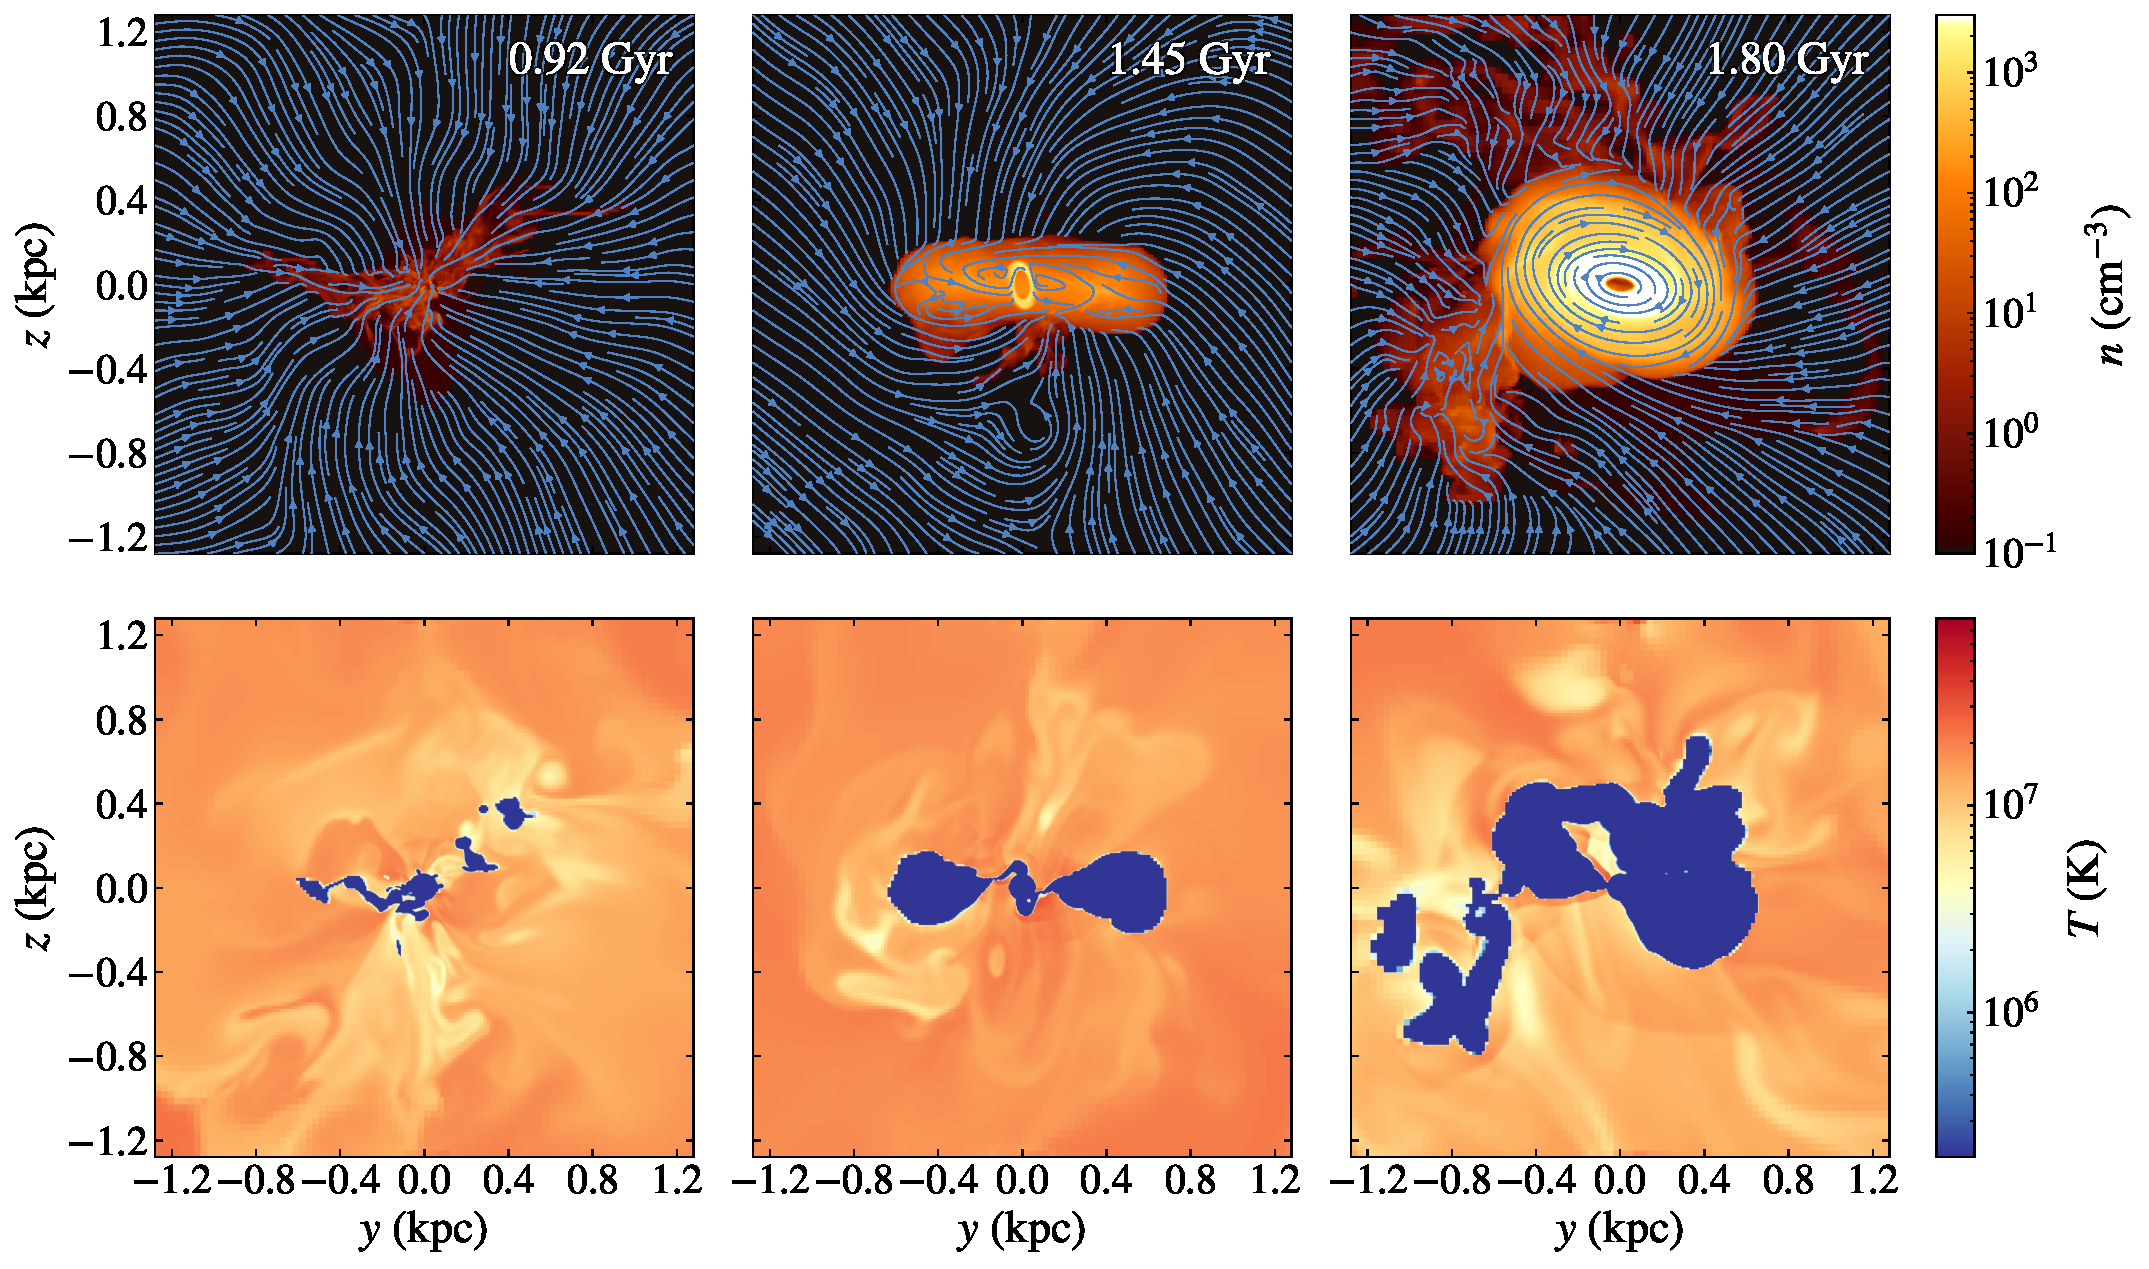
\includegraphics[width=\linewidth]{Sim_img/evolution_disk.pdf}
    \caption{Top: projections along the $x$-axis of the number density, $n$, at three timestamps: $t=920$\,Myr, $t=1450$\,Myr, and $t=1800$\,Myr. Blue streamlines denote the direction of gas flow. Bottom: $yz$-slices of temperature, $T$, at the same timestamps. At the sub-kpc scale, cool gas inflow transitions from filamentary to disky after $\sim 1$\,Gyr.\label{fig:thermodynamics}}
\end{figure}

\subsection{Multiphase gas evolution at the galaxy-scale}
\label{sec:galaxy-scale-result}

\subsubsection{The evolution of cool gas}

Throughout the 2\,Gyr evolution of the galaxy-scale simulation, cool gas precipitates from the hot halo through feedback-assisted thermal instability.
At times $t \lesssim 1$\,Gyr, the cool gas shows filamentary morphology, primarily oriented in the radial direction.
The cool gas cannot sustain ordered rotation because it does not carry enough angular momentum to allow circularization at the size of the accretion zone (see Section~\ref{subsec:filaments} for detailed discussion).
The left panels of Figure~\ref{fig:thermodynamics} show an instance of such a filamentary cool gas structure at time $t = 920\,$Myr.

After 1\,Gyr, the cool gas begins to carry enough angular momentum such that the gas circularizes around the accretion zone, creating a large-scale disk with a diameter reaching $\sim 1\,$kpc.
This disky phase is stable over time, but the disk itself precesses and becomes denser at the core ($n \sim 10^3$--$10^4\,\mathrm{cm^{-3}}$) over time, as can be seen in the middle and right panels of Figure~\ref{fig:thermodynamics}.
We also observe distinct layers of the disk rotating in different (sometimes opposite) directions at various points during this disky phase. The transition from an early filamentary cool structure to a cool disk at $\sim 1$\,Gyr is commonly seen in the jet-feedback simulations of \citet{li_2014a} and \citet{wang_agn_2019}.


\subsubsection{The hot gas}

Throughout the duration of the galaxy-scale simulation, hot gas exists in a quasi-steady state.
The hot gas thermodynamic profiles ($T$, $n$, and $P$) remain consistent with their initial profiles for most of the 2 Gyr evolution (see Figure~\ref{fig:r-prof-meso}).
The average luminosity of the jet is $L \equiv \dot{E}_{\rm jet} \approx 5 \times 10^{41}\, \mathrm{erg\,s^{-1}}$, which is comparable to the \textit{Chandra} X-ray luminosity of the central $\sim 10$\,kpc, but is several times smaller than the cooling luminosity of the entire galaxy.
This value is also in line with measurements of the jet power obtained from M87's multiwavelength spectral energy distribution \citep[SED,][]{prieto_central_2016}, but is one to two orders of magnitude lower than other estimates using X-ray cavity power \citep[e.g.,][]{forman_reflections_2005,russell_radiative_2013} or internal pressure exerted by knots in the jet \citep[e.g.,][]{owen_m87_2000,stawarz_dynamics_2006}.

The hot gas accretes primarily radially onto the inner boundary, with a very small rotational component ($v_{\rm r} \gtrsim 10^3\,v_{\rm rot}$, see also the velocity streamlines in Figure~\ref{fig:thermodynamics}).
The hot gas inflow rate through the inner boundary, $R_{\rm acc,R8} \approx 65$\,pc, is significantly smaller than the cool-gas inflow rate ($\dot{M}_{\rm in,cool} \gtrsim 10\,\dot{M}_{\rm in,hot}$) throughout the 2 Gyr evolution of the galaxy-scale simulation.


\begin{figure}
    \centering
    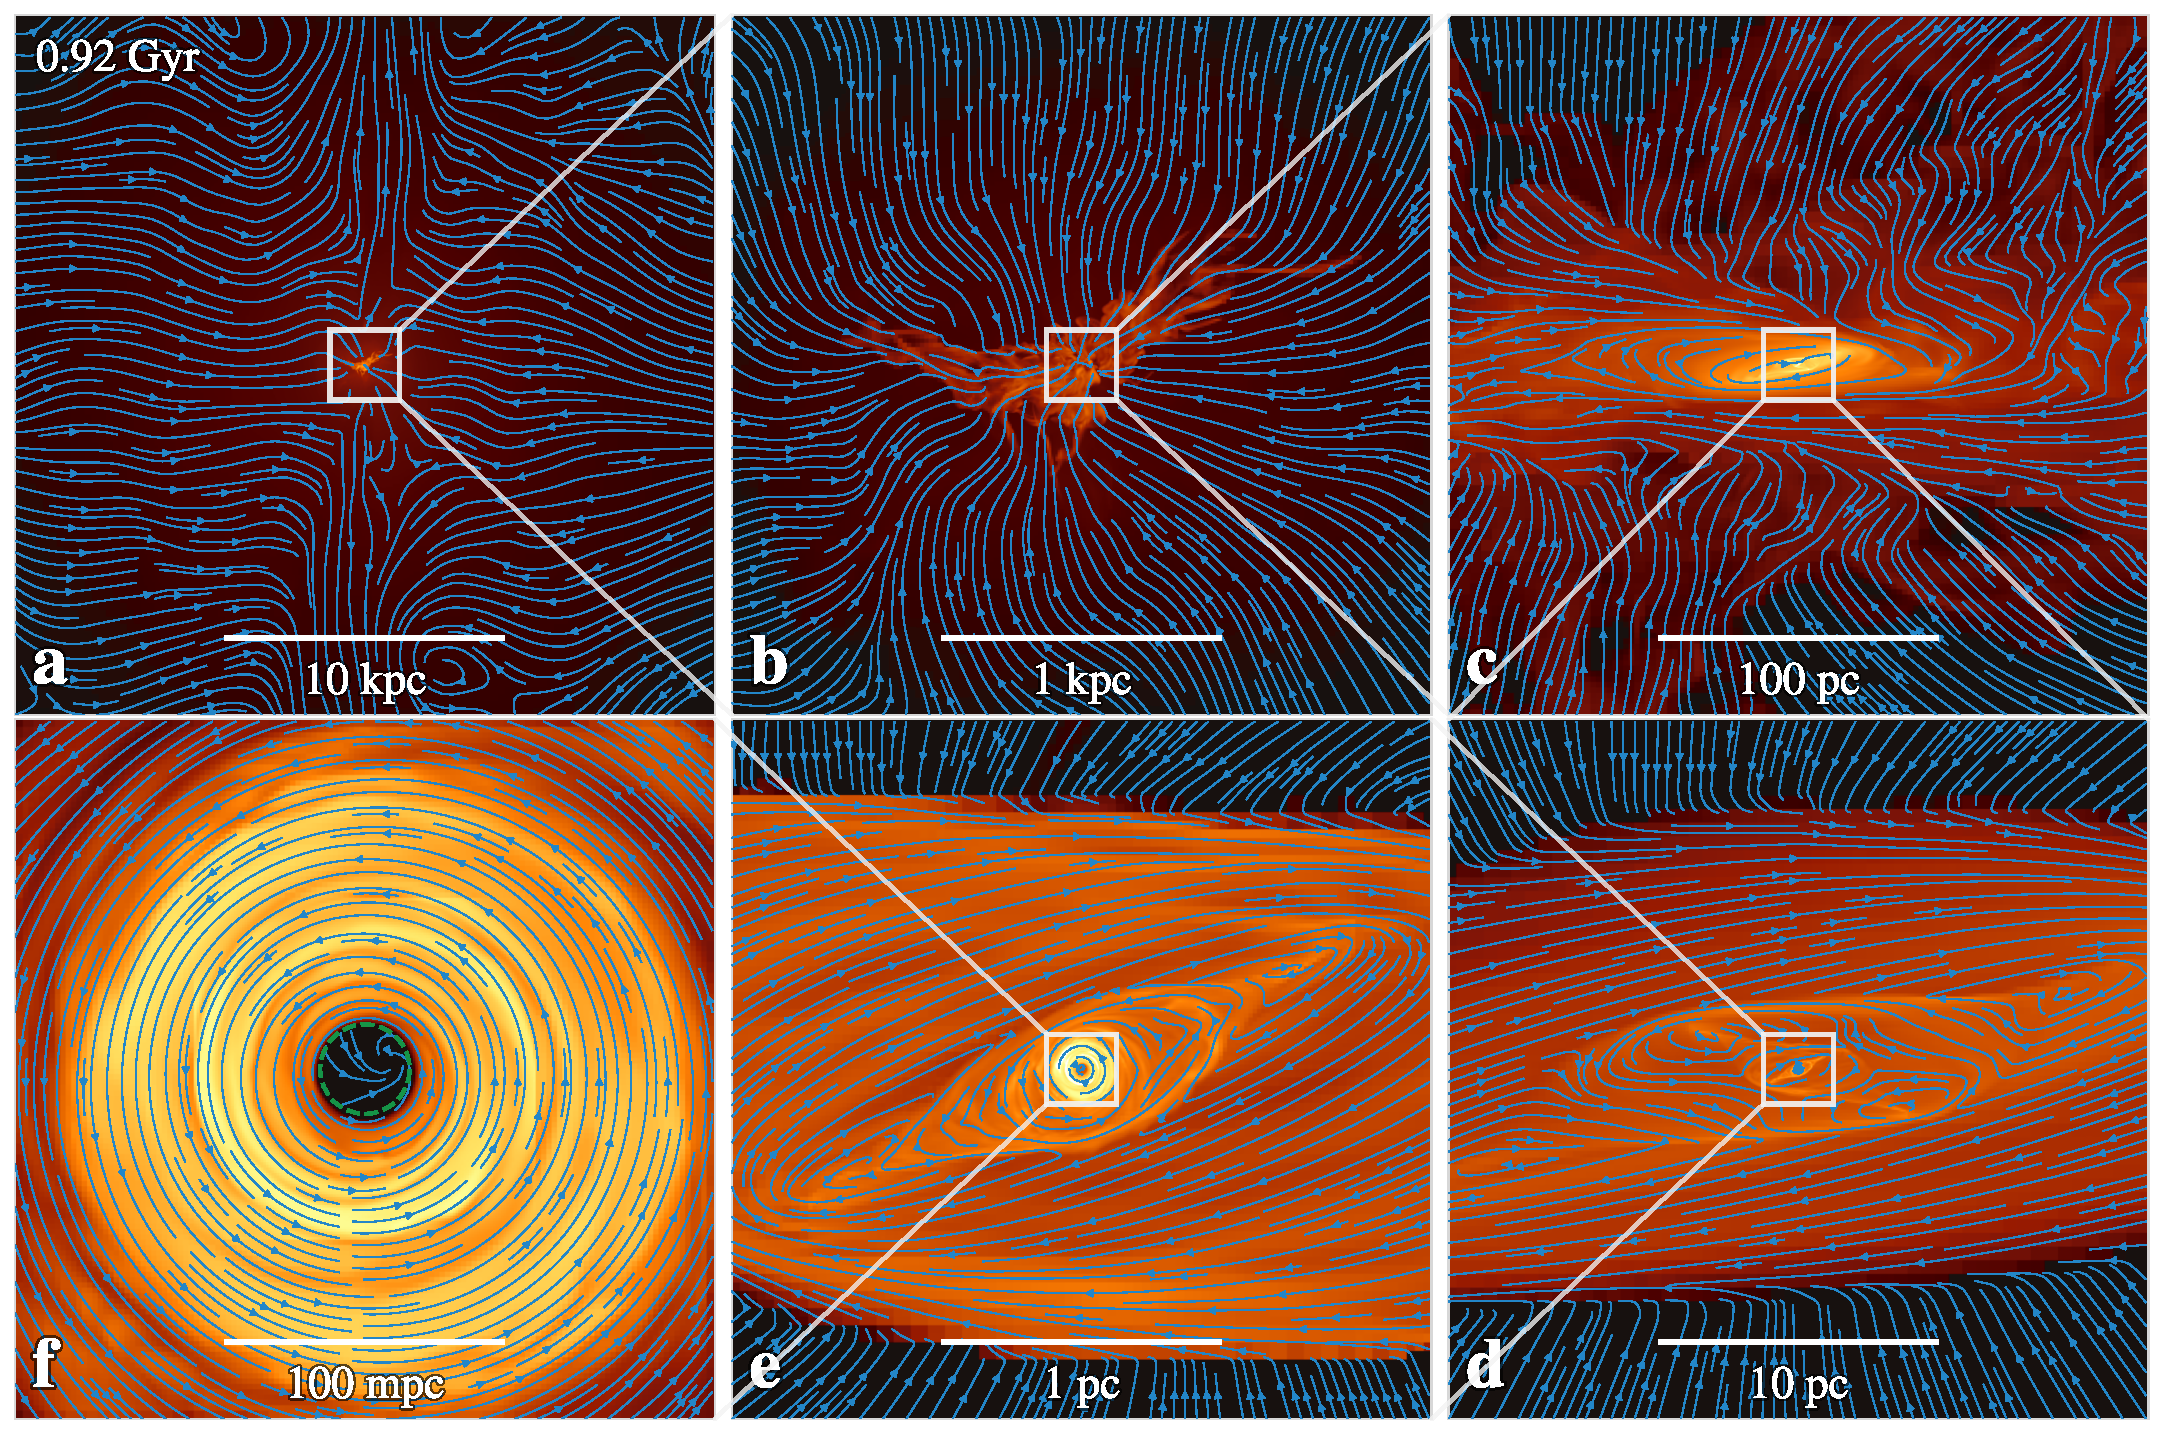
\includegraphics[width=\linewidth]{Sim_img/density_zoom_920Myr.pdf}
    \caption{Projections along the $x$-axis of the density at time $t\approx 920\,$Myr. Each panel is a $10\times$\ zoom of the previous panel, showing the cool gas morphology at various scales. Blue streamlines denote the direction of gas flow, while the green dashed circle in panel (f) denotes the extent of the accretion zone. The color scales are logarithmic, and are dynamically adapted to show features at each scale. At the largest scale, $10^{-2}\,\mathrm{cm^{-3}} < n < 10^2\,\mathrm{cm^{-3}}$. At the smallest scale, $10^{6}\,\mathrm{cm^{-3}} < n < 10^8\,\mathrm{cm^{-3}}$. \label{fig:zoom-in-proj}}
\end{figure}

\subsection{The meso-scale gas dynamics}
\label{sec:zoom-in-result}

We run a series of six zoom-in simulations starting from a galaxy-scale
snapshot to study the meso-scale gas dynamics. In this section, we describe the multiphase gas morphology, thermodynamics, and inflow/outflow rates. The results shown here are from our fiducial zoom-in at $t_{\rm restart} = 920\,$Myr.

\subsubsection{The multi-scale morphology of the cool gas}

Regardless of the galaxy-scale structure, the sub-100-pc cool gas exists within a coherent flow, taking the form of a disk (Figure~\ref{fig:zoom-in-proj}c-f).
The gas circularizes into a disk at a distance:
\begin{equation}
    r_{\rm circ} = \frac{\ell^2}{GM_{\rm BH}},
\end{equation}
where $\ell$\ is the specific angular momentum.
As the accretion zone is resolved at increasingly smaller scales ($R_{\rm acc,R8} \approx 4 \times 10^{3} R_{\rm acc,R20}$), the cool gas is much more likely to have $r_{\rm circ} > R_{\rm acc}$, making meso-scale cool disk formation highly probable. We discuss the effects of the accretion zone size on disk formation and stability in Section~\ref{subsec:filaments}.

The meso-scale disk exhibits dynamic structure across multiple spatial and temporal scales, with distinct gas layers oriented at different angles that continuously evolve as material accretes. Figure~\ref{fig:zoom-in-proj} shows an example snapshot of this multi-layered structure.
At the $\sim 100$\,pc scale, the outer disk is only starting to form from infalling kpc-scale filaments (Figure~\ref{fig:zoom-in-proj}c).
Inside this distance, the disk is thin and warped, and precesses around the $z$-axis.
The warped disk morphology extends two orders of magnitude in scale, from $\sim 50\,$pc to $\sim 0.5\,$pc (Figure~\ref{fig:zoom-in-proj}d-e).
Finally, the cool gas flow transitions to a face-on disk inside $\sim 0.5\,\mathrm{pc} \approx 10^3$\,\rg\ when viewed along the $x$-axis (Figure~\ref{fig:zoom-in-proj}f).

\begin{figure}
    \centering
    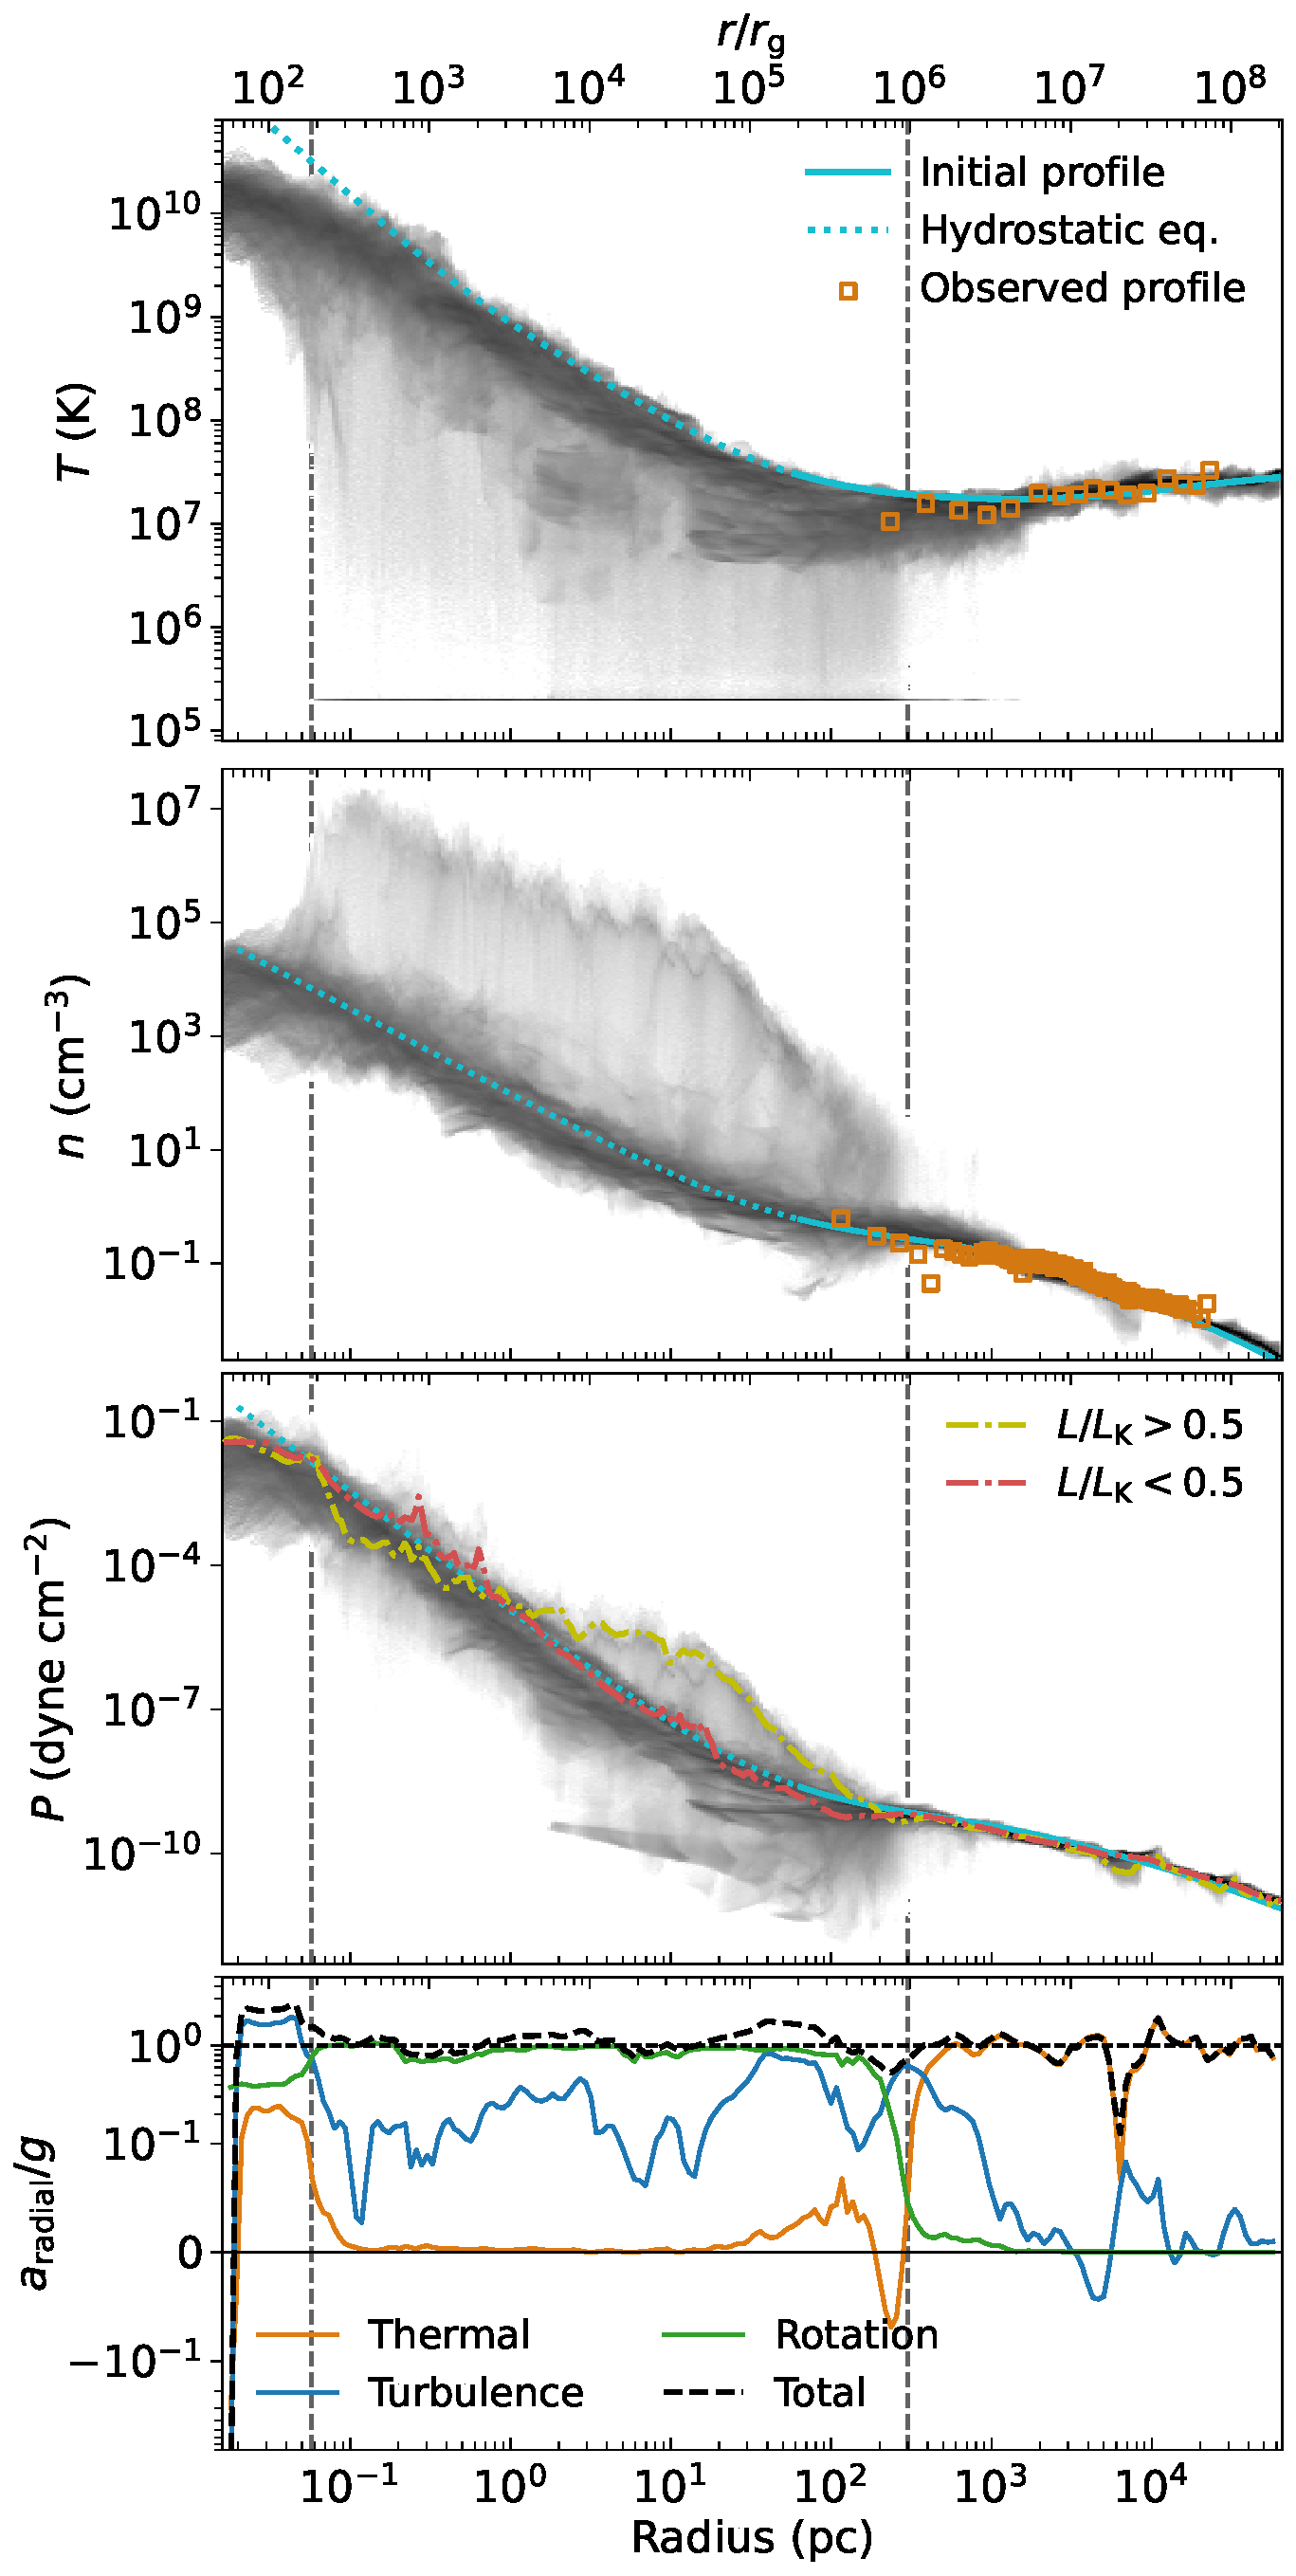
\includegraphics[height=0.65\textheight,keepaspectratio]{Sim_img/thermodynamics.pdf}
    \caption{Top three panels: temperature, number density, and pressure distributions, normalized at each radial bin, for the R20 simulation at $t\approx930\,$ Myr. Orange squares trace Chandra observations of M87, adapted from \citet{russell_inside_2015}. Solid teal lines are the initial profiles, and dotted teal lines are the extended profiles assuming hydrostatic equilibrium where $n(r = 2\,\mathrm{kpc}) = 0.1 \,\mathrm{cm}^{-3}$. The red and yellow lines in the pressure plot trace the mass-weighted profiles of the radially-dominated ($L/L_{\rm K} < 0.5$) and rotationally-dominated ($L/L_{\rm K} > 0.5$) gas, respectively.
    Bottom panel: radial acceleration from thermal pressure, turbulence pressure, and rotation, normalized by gravity, following the framework detailed in \citet{lochhaas_figuring_2022}. Positive values denote radially outward forces (against gravity). A total value of 1 signals radial force balance. The two vertical lines at $r=5.7\times10^{-2}$\,pc and $r=3\times10^{2}$\,pc mark the length scales where cool gas is rotationally supported within cool disks.\label{fig:r-prof-meso}}
\end{figure}

\subsubsection{The thermodynamics of the multiphase gas}

The bulk of the multiphase gas remains close to radial force balance after $\sim 1$\,Gyr.
Although a dense cool component precipitates out of the hot halo, the temperature ($T$), density ($n$), and pressure ($P$) profiles of the hot phase closely follow the initial hydrostatic solution, as obtained from the equations in Section~\ref{subsec:init}, over most scales (see Figure~\ref{fig:r-prof-meso}).
Since the volume-filling hot gas moves primarily in the radial direction, while the cool gas is rotationally supported, we separate the two types of motion by an angular momentum threshold, $L/L_{\rm K} = 0.5$ (where $L_{\rm K}$ is the Keplerian angular momentum) and compute the mass-weighted pressure profile of each type.
The radially-dominated gas practically overlaps with the initial hydrostatic equilibrium solution, while the rotationally-dominated gas deviates significantly from the hydrostatic equilibrium solution at length scales where cool gas is found (third panel of Figure~\ref{fig:r-prof-meso}).


The cool gas acts as an additional component embedded within the mostly hydrostatic hot atmosphere.
Its characteristic density is much higher than that of the hot gas at the same radii, but the maximum value is controlled by the imposed temperature floor, roughly following $n_{\rm cool} \sim \frac{P_{\rm hot}}{k_{\rm B}T_{\rm floor}}$.
A large fraction of the cool gas is at the floor temperature, $T =2\times10^5\,K$, with a smaller fraction ($\sim 40\%$) spanning intermediate temperatures $2\times10^5\,K < T < 10^7\,K$ as it mixes with the hot phase.


To understand the gas's radial force balance across scales and the physical processes responsible for supporting the galaxy against gravitational collapse, we adopt a procedure similar to \citet{lochhaas_figuring_2022} to compute the relative contribution of the different forces acting on the multiphase gas.
Briefly, we consider four support terms: thermal pressure, turbulent pressure, ram pressure, and rotation.
For each component, we compute the radial acceleration it provides against $\mathbf{g}$ and plot these values in the bottom panel of Figure~\ref{fig:r-prof-meso}:
\begin{equation}
\frac{F_{\rm total}}{m_{\rm gas}}
=
-\frac{1}{\rho}\frac{dP_{\rm th}}{dr}
-\frac{1}{\rho}\frac{dP_{\rm turb}}{dr}
-\frac{1}{\rho}\frac{dP_{\rm ram}}{dr}
+\frac{v_{\rm rot}^{2}}{r}.
\end{equation}
The first term is computed from the thermal pressure.
The second term is obtained first by smoothing the velocity field on the driving scale of turbulence ($54$\,kpc), then by calculating the residual velocity as the turbulent velocity:
\begin{equation}
    v_{\rm turb}^2 = \frac{1}{3}
[(v_x - v_{x,sm})^2
+
(v_y - v_{y,sm})^2
+
(v_z - v_{z,sm})^2],
\end{equation}
where $v_{x,sm}$, $v_{y,sm}$, and $v_{z,sm}$ are the smoothed velocity fields in Cartesian directions.
Then, the turbulent pressure is:
\begin{equation}
    P_{\rm turb} = \rho_{sm} v_{\rm turb}^2.
\end{equation}
The third term is computed from the smoothed radial velocity field, $v_{r,sm}$:
\begin{equation}
    P_{\rm ram} = \rho_{sm} \left(\frac{dv_{r,sm}}{dr}\Delta x\right)^2,
\end{equation}
where $\Delta x$ is the cell size of the grid.
In practice, we find that ram pressure contributes negligibly to the overall force budget of the system, so we ignore its effects in our analysis.
Lastly, the rotational force is computed as:
\begin{equation}
    \frac{v_{\rm rot}^2}{r} = \frac{v_{\theta,sm}^2 + v_{\phi,sm}^2}{r},
\end{equation}
where $v_{\theta,sm}$ and $v_{\phi,sm}$ are the smoothed tangential velocity components.



In the R20 simulation, we find that the three components of radial force add up to approximately balance gravity over most radii. At kpc scales, thermal pressure is the dominant factor.
Then, as cool gas forms at the kpc scale and undergoes ordered rotation around $300\,\mathrm{pc}\approx 10^6\,r_{\rm g}$, the main source of radial force transitions from thermal pressure to rotation.
Turbulent support is negligible at large scales, remains small but measurable between $10^{-1}$\,pc and $\sim 100$\,pc, before becoming the dominant component below $10^{-1}$\,pc.
These two transitional scales correspond first to the formation of cool gas, then to the disappearance of cool gas near the SMBH.


\subsubsection{The kinematics of the multiphase gas: inflow, outflow, and rotation} \label{subsec:m-dot-scaling}

We compute the mass inflow and outflow rates through spherical shells to understand the mass accretion rate's dependence on radius.
For each cell within a radial bin, the mass flux through it is:
\begin{equation}
    \Phi_{\rm M} = v_r \cdot \rho,
\end{equation}
where $v_r$\ is the radial velocity and $\rho$\ is the gas density.
Then, these cells are separated into four categories depending on the local temperature and the direction of the radial velocity: hot inflow, hot outflow, cool inflow, and cool outflow.
The inflow/outflow determination is based on a cell's velocity vector pointing toward or away from the center of the domain (the SMBH).
For example, a cell with a temperature $T_{\rm cell} < 10^6$\,K and a radial velocity $v_{r, \,\rm cell} > 0$\ is classified as ``cool outflow''.
Then, the mass flow rate is computed as the mass flux through the surface of a sphere:
\begin{equation} \label{eq:accretion-from-flux}
    \dot{M} = 4 \pi r^2 \Phi_{\rm M} = 4 \pi r^2 v_r \rho.
\end{equation}

Because of how we define inflow/outflow, if gas is in an elliptical disk, the computed inflow and outflow rates would both be non-zero due to the radial velocity component within the disk.
Therefore, we use the net inflow rate, ``net $\dot{M}_{\rm in}$'', which tracks the overall accretion rate at each radial bin.
We plot these properties at time $t \approx 930$\,Myr, averaged over 1\,kyr, in the top panel of Figure~\ref{fig:l-m-dot-meso}.

The hot and cool phases show distinct accretion behavior across scales.
The cool gas inflow and outflow rates are comparable across the resolved radii because it predominantly settles into rotationally supported disks.
Meanwhile, the hot outflow rate is comparable to the inflow rate at $\gtrsim 1$\,kpc scales, falling to $1\text{--}2$ orders of magnitude lower than inflow over $\sim 1$--$10^3$\,pc.
The average net \mdot, represented by purple dots in the upper panel of Figure~\ref{fig:l-m-dot-meso}, is consistent with a power law across the dynamic range.
At this time, the accretion rate follows:
\begin{equation} \label{eq:930_scaling}
    \dot{M}_{\rm in}\,[M_{\odot}\,\mathrm{yr^{-1}}] \approx 0.16\, (r\,\mathrm{[pc]})^{0.40}.
\end{equation}
The slope is not universal throughout our simulations, however.
At $t\approx1460$\,Myr, $\dot{M}\propto r^{0.61}$, and at $t\approx1510$\,Myr, $\dot{M}\propto r^{0.69}$.
Given the limited number of meso-scale simulations available, we cannot make definitive statements about how differing gas morphologies dictate the slope of this relation.
Nevertheless, our result is in line with the \mrrelation\ relation found in multiple numerical studies of similar low-accretion-rate systems \citep[e.g.,][]{ressler_ab_2020,white_structure_2020,lalakos_bridging_2022,guo_toward_2023,guo_magnetized_2024, cho_multizone_2024}.

Our estimate of the Bondi accretion rate at this time is $\dot{M}_{\rm B} \approx 0.74\,M_{\odot}\,\mathrm{yr^{-1}}$, which is higher than observational estimates of $\approx 0.1\,M_{\odot}\,\mathrm{yr^{-1}}$\ \citep{di_matteo_accretion_2003,russell_inside_2015}.
However, see Section~\ref{sec:bondi-discussion} for a more in-depth discussion of the factors contributing to such a discrepancy.
For now, we note that \mdotb\ is virtually equal to the net inflow rate of the hot gas at that scale.

Notably, both the inflow and outflow rates of cool gas drop to effectively zero below $\sim 100$\,\rg.
This behavior matches the thermodynamic profiles in Figure~\ref{fig:r-prof-meso}, which show cool gas disappearing below $\sim 6 \times 10^{-2}$\,pc $\approx 200\, r_{\rm g}$.
We also observe a consistent flattening of the net \mdot\ profile at $r \lesssim 100\,r_{\rm g}$ across the three simulations, supporting our assumption in calculating the true \mdotbh\ values from the galaxy-scale simulation (Equation~\ref{eq:scaling}).

\begin{figure}
    \centering
    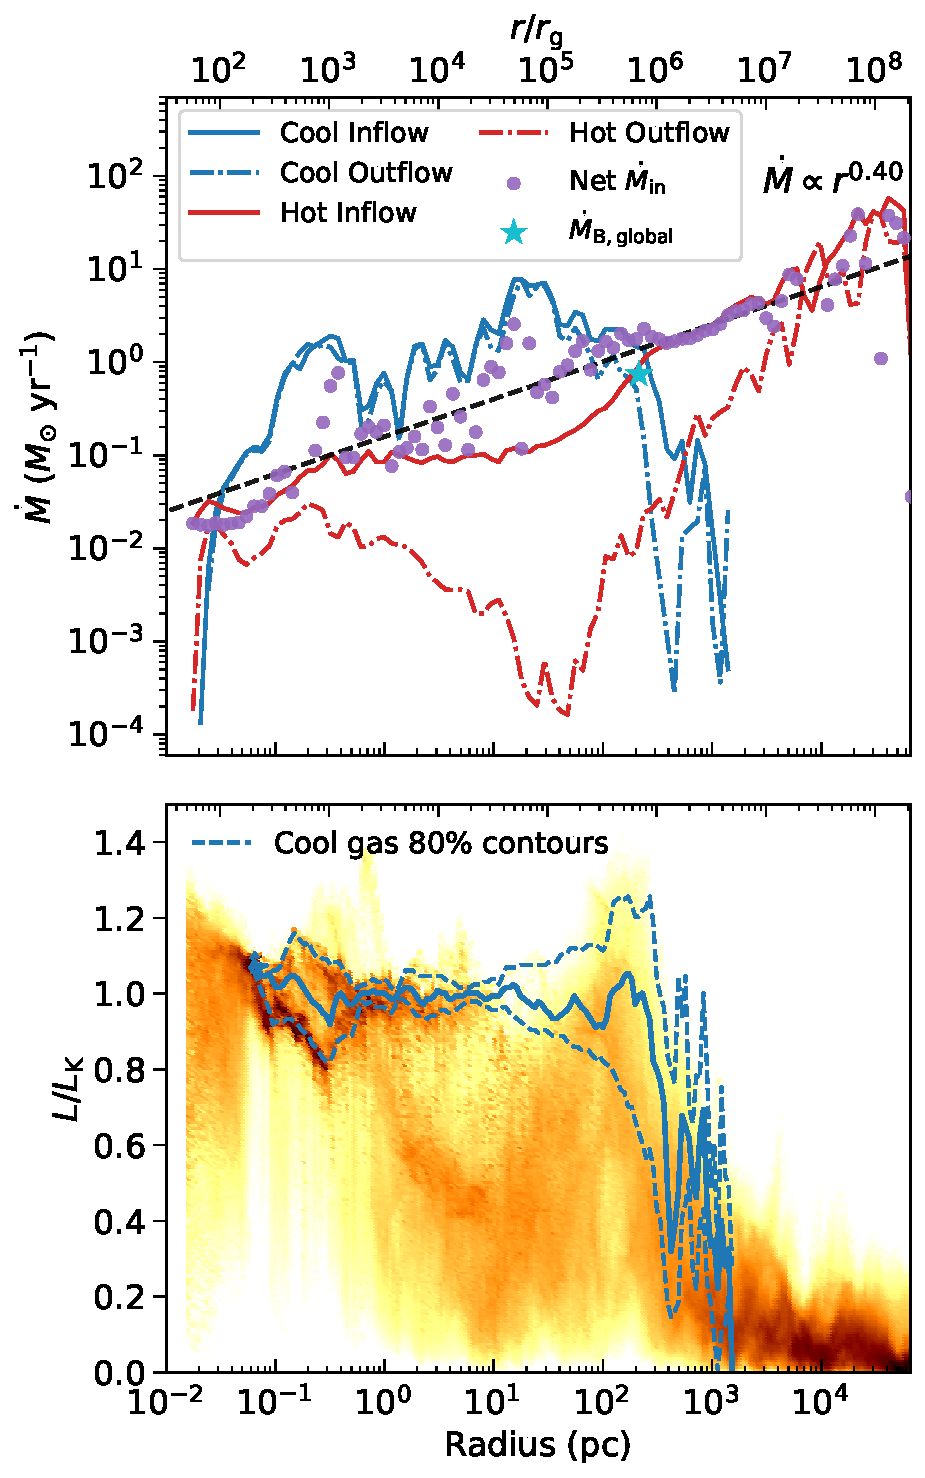
\includegraphics[height=0.65\textheight,keepaspectratio]{Sim_img/angular-momentum_m-dot_930.pdf}
    \caption{Top: Inflow/outflow rates of the multiphase gas. The inflow component is plotted in solid lines, while the outflow component is in dotted-dashed lines. Purple dots are the net inflow, and the black dashed line is a fit for the net inflow, which follows the relation $\dot{M} \propto r^{0.40}$. The teal star shows the global Bondi accretion rate of the system (\mdot$_{\rm B,global}$, see Section~\ref{sec:bondi-discussion}), which is roughly equal to the net inflow rate of hot gas at the same radius. Bottom: Distribution of hot gas total angular momentum, normalized by the Keplerian angular momentum ($L/L_{\rm K}$). Darker shades indicate higher fractions of gas at each radial bin. Blue solid line is the cool gas mass-weighted angular momentum radial profile, bracketed by two dashed lines that represent the 10th and 90th percentiles of the cool-gas distribution.\label{fig:l-m-dot-meso}}
\end{figure}

\begin{figure}
    \centering
    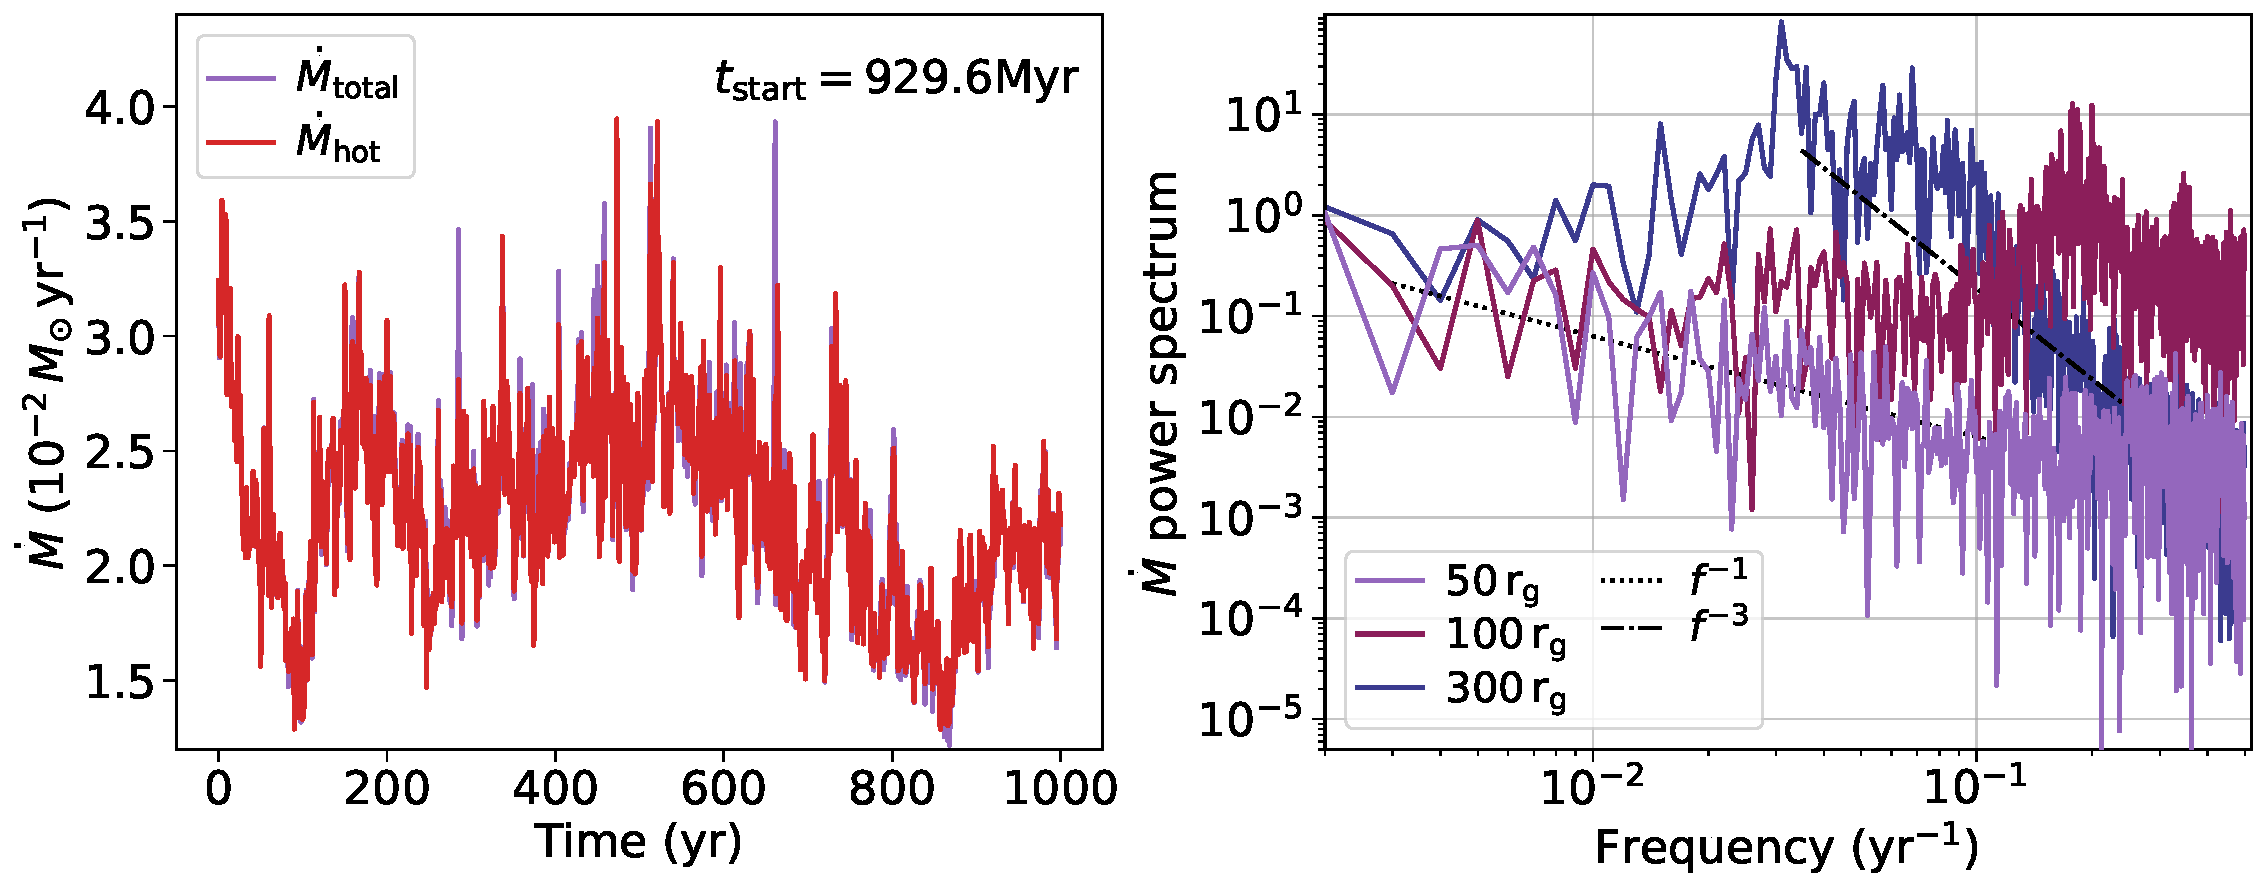
\includegraphics[width=\linewidth]{Sim_img/mdot_meso_930.pdf}
    \caption{Left: \mdot\ measured at the inner boundary, $R_{\rm acc,R20}\approx 16$\,mpc $\approx 50\,r_{\rm g}$, of the hot gas (red) and total gas (purple). Virtually all cool gas has been compression-heated into the hot phase, so the cool gas accretion rate is regularly $\gtrsim 2$\ orders of magnitude below the hot gas accretion rate. We have therefore omitted the line here for clarity. Right: power spectrum of \mdot, measured at $r \approx 50\,r_{\rm g} \approx R_{\rm acc,R20}$ (purple), at $r = 100\,r_{\rm g} \approx 31$\,mpc (magenta), and at $r = 300\,r_{\rm g} \approx 0.1$\,pc (dark blue). The dotted and dotted-dashed lines are reference slopes for the spectra.\label{fig:m-dot-meso}}
\end{figure}

We also examine the motion of the cooling flow through its angular momentum distribution in the lower panel of Figure~\ref{fig:l-m-dot-meso}.
The cool gas does not exist in significant quantities beyond $r \sim 2$\,kpc.
Cool gas initially possesses low angular momentum as it precipitates out of the hot halo ($L_{\rm cool}/L_{\rm K}\approx0.4$), before settling onto rotationally supported disks inside $\sim 200$\,pc.
The cool gas remains in Keplerian disks ($L_{\rm cool}/L_{\rm K}\approx1$) all the way until it disappears at $\sim 6\times10^{-2}$\,pc.

At large scales, $r\gtrsim 1$\,kpc, the hot gas motion is predominantly radial ($L_{\rm hot}/L_{\rm K} \lesssim 0.2$).
Inside $\sim 1$\,kpc, hot gas is found with a wide range of angular momentum, with a roughly uniform spread in the range $0 < L_{\rm hot}/L_{\rm K} \lesssim 1$.
At $1\,\mathrm{pc} \lesssim r \lesssim 200$\,pc, the hot and cool phases are kinematically decoupled.
Inside $r \sim 5\times10^3\,r_{\rm g} \approx 1\,$pc, the two phases begin to overlap in angular-momentum space, as can be seen by the cospatiality between the hot gas angular momentum distribution and the 80th-percentile contours of the cool gas in Figure~\ref{fig:l-m-dot-meso}.
At these scales, gas from the cool disk is heated above the $10^6\,K$ threshold, turning into hot gas, while retaining substantial rotational support.
This heating process concludes at $\sim 6\times10^{-2}\,$pc, where the cool phase is completely depleted.
Inside this scale, the hot gas angular-momentum distribution spreads out more widely, spanning $0 < L_{\rm hot}/L_{\rm K} \lesssim 1.3$.

\subsubsection{Accretion variability} \label{subsec:variability}

We study both the total accretion rate through the smallest accretion zone ($R_{\rm acc,R20}=4^2\,\mathrm{mpc}\approx 50\,r_{\rm g}$) and its associated variability in this subsection. For this analysis, we rerun the meso-scale simulation (R20) at $t\approx930$\,Myr and record the accretion rate with a one-year cadence, over $\Delta t = 1$\,kyr.
Throughout this period, we observe no significant variability in the accretion rate, with at most a factor of $\sim 2$ difference in \mdotbh\ (see the left panel of Figure~\ref{fig:m-dot-meso}).
The low variability agrees with multi-year X-ray observations of M87 \citep[][]{prieto_central_2016,cheng_year-scale_2023}.
Given an average \mdotbh\ over this period of $\approx 2.2\times10^{-2}\, \mathrm{M_{\odot}\,yr^{-1}}$, the inferred jet power, using Equation~\ref{eq:jet_power} with $\eta \approx 10^{-4}$, is $\mathcal{P}_{\rm jet} \approx 10^{41}\,\mathrm{erg\,s^{-1}}$.

We estimate the AGN jet variability by computing the $\dot{M}$\ power spectrum at three distances from the SMBH in the meso-scale simulation: (1) at the inner boundary, $r = R_{\rm acc,\,R20}\approx 50\,r_{\rm g}$, (2) at $r = 100$\,\rg, and (3) at $r = 300$\,\rg\,$\approx 0.1\,$pc, and plot them in the right panel of Figure~\ref{fig:m-dot-meso}.

At the accretion zone, the power spectrum is shallow, approximately $S\propto f^{-1}$, indicating weak variability in \mdot, and thus in the jet power, over the 1\,kyr evolution. The same behavior is also observed in the time series shown in the left panel. At $r=100$\,\rg, the spectrum has a different shape: it steepens to $S\propto f^{-3}$ at high frequencies ($f\gtrsim0.1\,\mathrm{yr^{-1}}$), but flattens at lower frequencies. This suggests that the accretion rate varies on short, year-to-decade timescales, while remaining comparatively stable over longer timescales. The same radius also marks the flattening of the \mdot\ radial profile (see Figure~\ref{fig:l-m-dot-meso}).
At $r = 300$\,\rg\,$\approx0.1$\,pc, the power spectrum remains at a steep $-3$ slope over a larger range of frequencies.
The $f^{-3}$ portion appears to extend to lower frequencies as the measurement radius increases.
Overall, however, it is difficult to ascertain the significance of the results at these scales due to the many potentially important physical processes not accurately captured by our hydrodynamic simulation, such as magnetic and relativistic effects.
We discuss these limitations in further detail in Section~\ref{subsec:limitations}.

\subsection{Discussion} \label{sec:discussion}

\subsubsection{Bondi accretion model in the context of multiphase, inhomogeneous accretion} \label{sec:bondi-discussion}

\begin{figure}
    \centering
    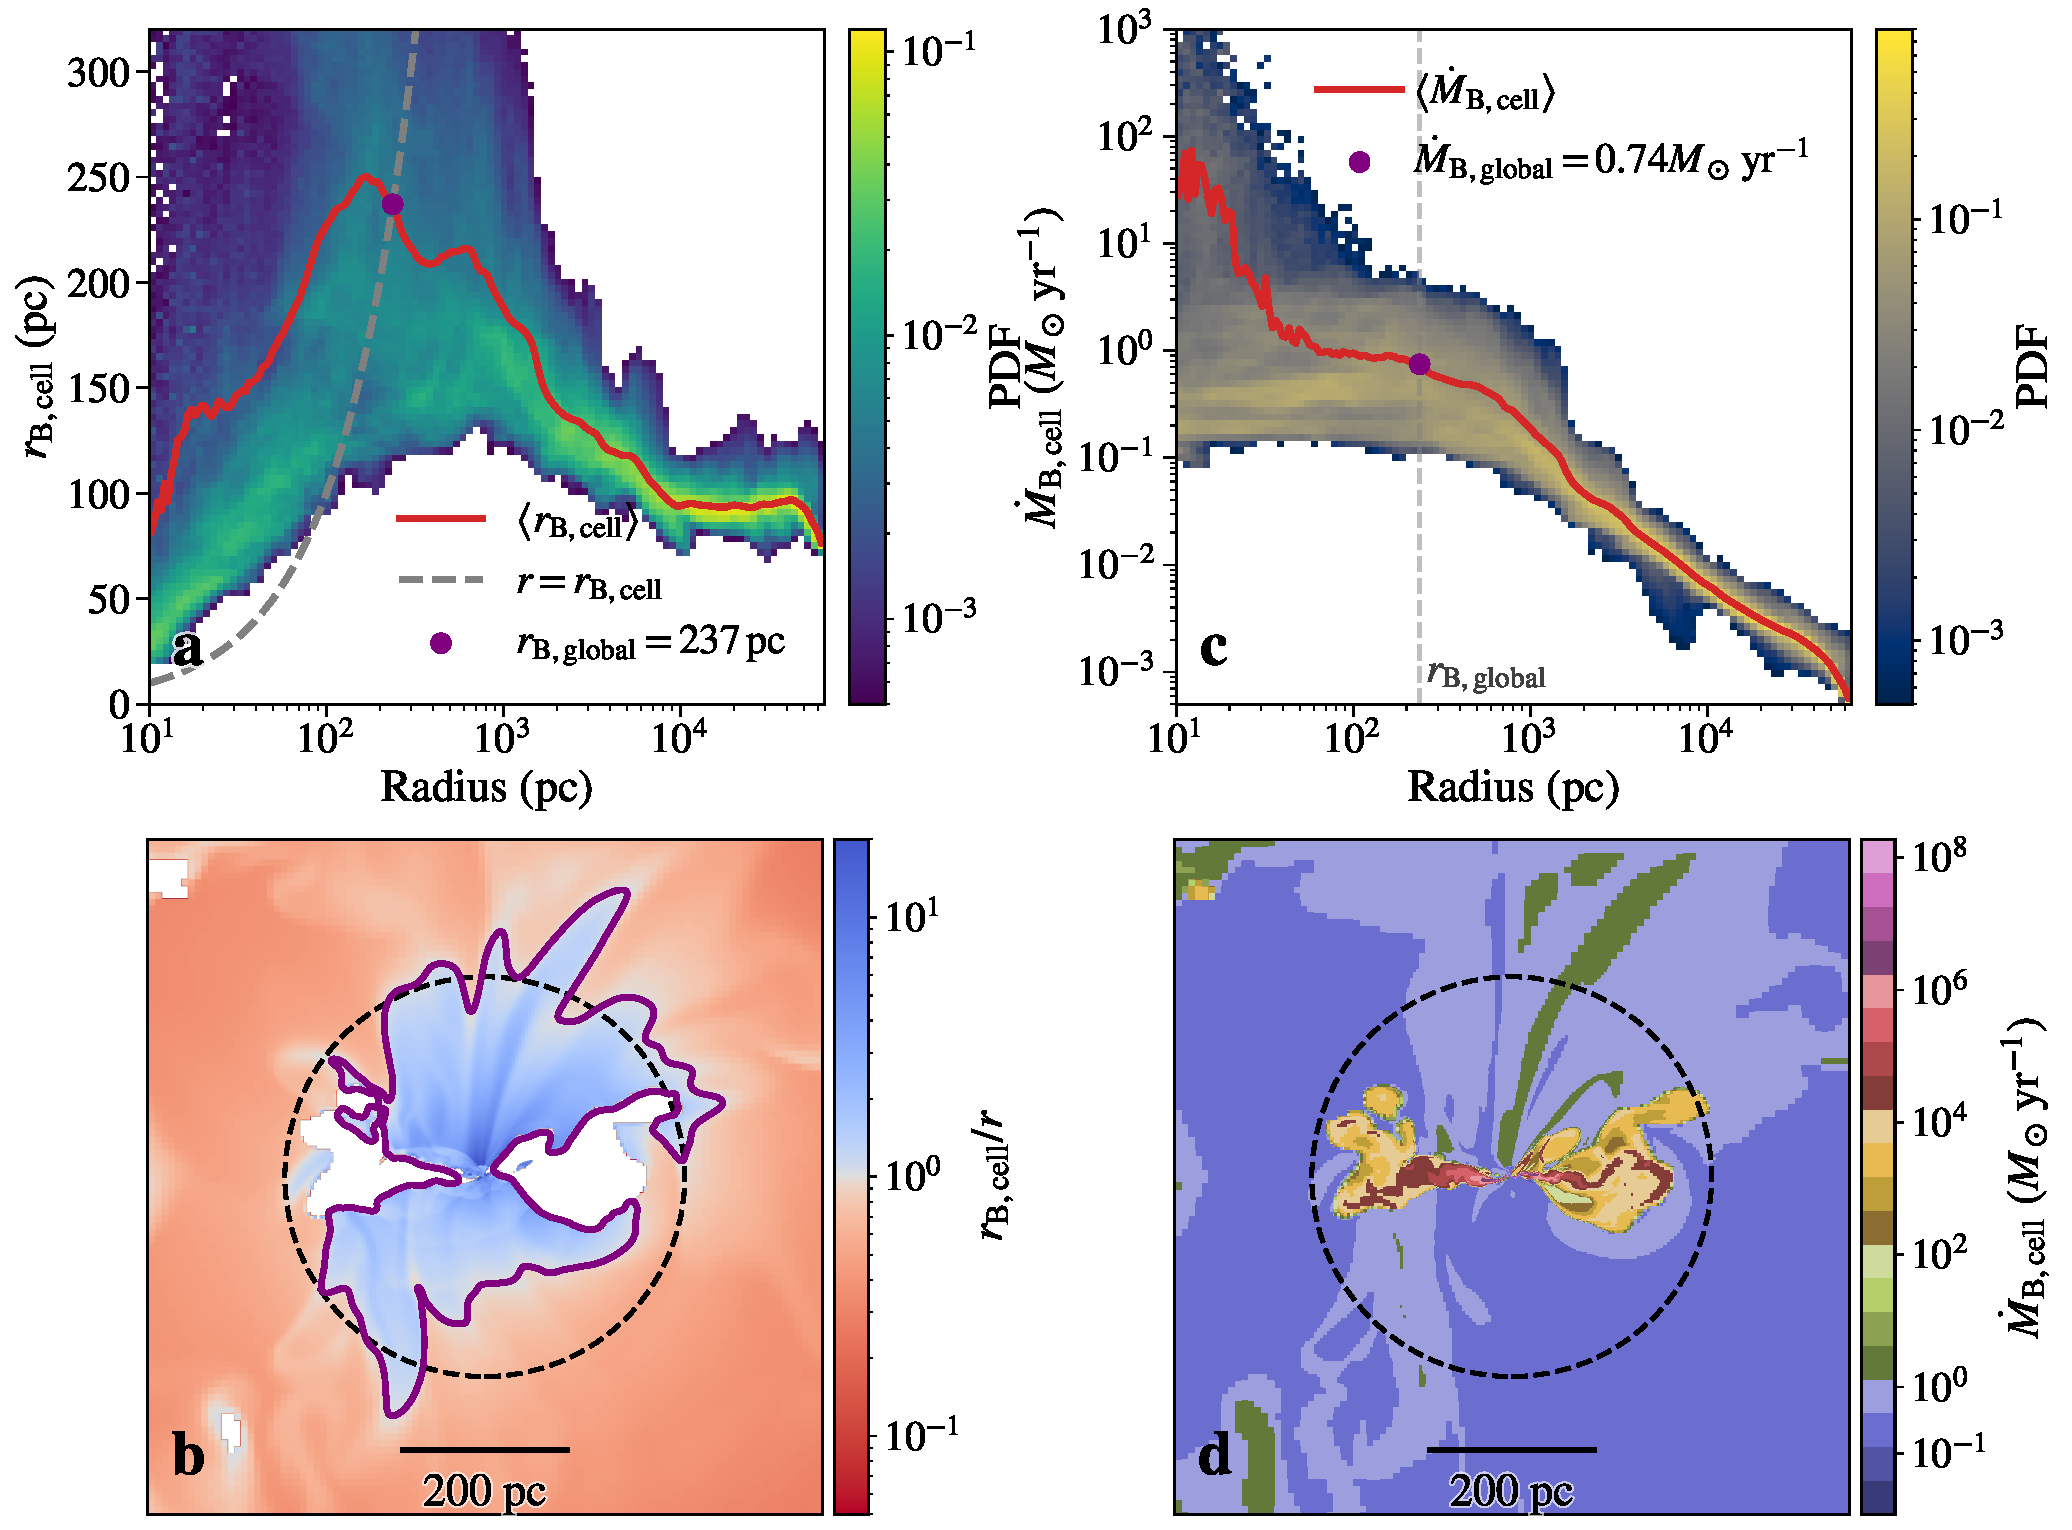
\includegraphics[width=\linewidth]{Sim_img/bondi_analysis_930.pdf}
    \caption{(a) Probability density function, normalized by each radial bin, of the cell-level Bondi radius (following Equation~\ref{eq:rb}) as a function of distance from the black hole. The red line shows the mass-weighted average ($\langle r_{\rm B,cell}\rangle$) radial profile. We approximate a global Bondi radius of the system as the location where $\langle r_{\rm B,cell}\rangle = r = 237$\,pc (purple dot).
    (b) $yz$-slice plot of $r_{\rm B,cell}/r$, with gas below the Bondi-analysis temperature cut ($T < 5 \times 10^6\,\mathrm{K}$) masked out. The purple contour denotes the real Bondi surface of this system (where $r_{\rm B,cell}/r =1$), which is distinctly non-spherical compared to the black dashed circle of radius $r = r_{\rm B,global}$.
    (c) Same as (a), but for the cell-level Bondi accretion rate (following Equation~\ref{eq:m-dot-bondi}). We estimate a global Bondi accretion rate of the system as $\dot{M}_{\rm B,global} \equiv \langle \dot{M}_{\rm B,cell}\rangle (r=r_{\rm B,global}) = 0.74\,\mathrm{M_{\odot}\,yr^{-1}}$.
    (d) $yz$-slice plot of $\dot{M}_{\rm B,cell}$. The Bondi accretion rate in the hot phase is in line with observational expectations, $\dot{M}_{\rm B,\ hot} \sim 0.1\, \mathrm{M_{\odot}\,yr^{-1}}$.\label{fig:bondi-m-dot-r}}
\end{figure}

The classical Bondi accretion model assumes a spherically symmetric accretion flow of a single-phase medium onto a point mass---the SMBH at the center of a galaxy.
Within this accretion flow, there exists a distance from the black hole at which the escape velocity of the gas equals its sound speed.
This distance, the Bondi radius, is expressed as:
\begin{equation}\label{eq:rb}
    r_{\rm B} = \frac{2GM_{\rm BH}}{c^2_{s}},
\end{equation}
where $G$\ is the gravitational constant, $M_{\rm BH}$\ is the black hole mass, and $c_{s}$\ is the sound speed of the single-phase medium.
For the hot gas in M87, \textit{Chandra} measurements give a central temperature of $k_{\rm B}T \approx 0.9$\,keV, implying $r_{\rm B} \approx 120$--$220$\,pc \citep{russell_inside_2015}.

The Bondi accretion rate can be computed as the mass flux through the surface of the Bondi sphere:
\begin{equation}\label{eq:m-dot-bondi}
    \dot{M}_{\rm BH} \approx \dot{M}_{\rm B} = \frac{4\pi G^2 M^2_{\rm BH}\rho}{c^3_{s}}\,.
\end{equation}
In M87, the inferred Bondi accretion rate using the observed X-ray density and temperature is \mdotb\,$\approx 0.1\,\mathrm{M_{\odot}\,yr^{-1}}$\ \citep[][]{russell_inside_2015}.

\centerline{\textbf{The limitations of the traditional Bondi model}} \label{subsec:bondi-limit}

The Bondi model makes several key assumptions about the accretion flow that do not accurately reflect the environment around AGNs.

Firstly, observations have detected multiphase gas inside the Bondi radius in several nearby systems, both in \halpha\ \citep[e.g.,][]{conselice_nature_2001,boselli_virgo_2019} and the molecular phase \citep[e.g.,][]{combes_alma_2019, hsieh_circumnuclear_2021}.


Secondly, the hot phase is inhomogeneous, and hot accretion is rarely spherically symmetric. X-ray measurements of line widths toward cluster cores have suggested that the hot phase is turbulent \citep[e.g.,][]{zhuravleva_turbulent_2014,hitomi_collaboration_atmospheric_2018}. Significant outflows also originate from inside the Bondi radius, from both black hole feedback \citep[e.g.,][]{mcnamara_heating_2005} and stellar feedback \citep[e.g.,][]{hopkins_stellar_2016}.

Thirdly, the inflow rate of gas through the Bondi radius is much larger than the accretion rate onto the SMBH\@. In addition to outflows, cool gas clumps carry some angular momentum as they enter the Bondi sphere and form accretion disks \citep[e.g.,][]{walsh_m87_2013,hsieh_circumnuclear_2021}. The disk provides angular momentum support against infall, which slows down accretion. In M87, accretion rate measurements via the jet mechanical power \citep[][]{broderick_event_2015}, or from Faraday rotation at the nucleus of the galaxy \citep[][]{kuo_measuring_2014} showed that the accretion rate at the event-horizon-scale is two to three orders of magnitude lower than the Bondi accretion rate. The same discrepancy is also seen in multiple GRMHD simulations constructed to inform the EHT result \citep[][]{eht_eight}.


\centerline{\textbf{A new perspective on the ``Bondi sphere''}}

Using our multi-scale simulation, we examine the Bondi accretion model and discuss its applicability in a multiphase accretion flow.
Firstly, we use Equation~\ref{eq:rb} to compute the Bondi radius, $r_{\rm B,cell}$, for gas with $T \geq 5\times10^6\,\mathrm{K}$, equivalent to $k_{\rm B}T \geq 0.43$\,keV, in each grid cell.
We adopt this stricter temperature cut to isolate the gas near the virial temperature; cooler gas has a lower sound speed and therefore much larger values of both \rb\ and \mdotb.
Then, we present a range of $r_{\rm B,cell}$ values across radial distances with a phase plot in Figure~\ref{fig:bondi-m-dot-r}a.
At small radial distances, the spread in the $r_{\rm B,cell}$ values is large, corresponding to large fluctuations in the hot gas temperature.
Outside $r \sim 3$\,kpc, the distribution becomes less variable and settles around $r_{\rm B,cell}\,\approx 100$\,pc.

As one moves along a radial line toward the center, there comes a point in space where the inward gravitational force overtakes the outward force exerted by the thermal gas pressure.
We identify such a point by tracking the ratio between a cell's Bondi radius and its radial distance, $r_{\rm B,cell}/r$. The isosurface tracing $r_{\rm B,cell}/r = 1$\ is the true ``Bondi surface'' of the system.
We visualize this surface as a purple contour in Figure~\ref{fig:bondi-m-dot-r}b. The gas inside this boundary is expected to accrete at supersonic speed.
The Bondi surface replaces the Bondi sphere in a turbulent, inhomogeneous accretion flow.
We find the true Bondi accretion rate by computing the net inflow rate through this surface:
\begin{equation}\label{eq:true-mdotb}
    \dot{M}_{\rm B,surface} = -\oint_S \rho \mathbf{v}\cdot d\mathbf{A},
\end{equation}
where $\rho$\ is the gas density, $\mathbf{v}$\ is the velocity vector, and $d\mathbf{A}$\ is the outward-pointing area element. The inferred net accretion rate using Equation~\ref{eq:true-mdotb} is $\dot{M}_{\rm B,surface} = 1.2\,\mathrm{M_{\odot}\,yr^{-1}}$.


\centerline{\textbf{Estimating Bondi accretion rate with our proposed model}}

In practice, most modern cosmological simulations (as well as X-ray observations) are not able to resolve the complex morphology of the Bondi surface.
Nevertheless, we can still extract useful information about the accretion flow by approximating a Bondi radius of the whole system.
We obtain a mass-weighted radial profile of $r_{\rm B,cell}$ (Figure~\ref{fig:bondi-m-dot-r}a, red line), then define the global Bondi radius to be where $r = \langle r_{\rm B,cell} \rangle$\ (Figure~\ref{fig:bondi-m-dot-r}a, purple dot).
In the R20 simulation at $t\approx930$\,Myr, $r_{\rm B,global}=237$\,pc.
This value is approximately equal to a volume-equivalent radius of the Bondi region, $r_{\rm B,surface} = r[\int dV(r_{\rm B,cell}/r\geq 1)] = 214$\,pc.

We then use Equation~\ref{eq:m-dot-bondi} to compute the Bondi accretion rate of the hot gas cell-by-cell.
In contrast with the $r_{\rm B,cell}$ distribution, the distribution of $\dot{M}_{\rm B,cell}$ as a function of radius shows much less scatter and generally plateaus around $0.1$--$1\,\mathrm{M_{\odot}\,yr^{-1}}$ between $\sim10$\,pc and $10^3$\,pc.
This plateau can be explained by the relatively flat profiles of gas density and temperature over this scale range (see Figure~\ref{fig:r-prof-meso}).
\citet{li_simulating_2012} suggested that this flatness is a result of a self-regulated balance between adiabatic compression and cooling, and depends strongly on the gravitational profile of the stellar (brightest cluster galaxy) potential.
The global Bondi accretion rate, obtained by taking the mass-weighted value of $\dot{M}_{\rm B,cell}$ at $r_{\rm B,global}$, is $\dot{M}_{\rm B,global} = \langle \dot{M}_{\rm B,cell} \rangle \approx 0.74\,\mathrm{M_{\odot}\,yr^{-1}}$.
This value is within one order of magnitude of earlier estimates from \textit{Chandra} X-ray observations \citep{di_matteo_accretion_2003, russell_inside_2015}, and is also consistent with the true Bondi accretion rate of the system, $\dot{M}_{\rm B,surface} = 1.2\,\mathrm{M_{\odot}\,yr^{-1}}$.
However, one important distinction between our system and the Bondi model is that a large amount of cool gas contributes to the overall accretion flows, which dramatically boosts the inflow rate at the \rb\ scale (see Figure~\ref{fig:l-m-dot-meso}).
Even the new Bondi surface that we introduce here does not account for cool gas accretion.

To further emphasize the disconnect between the Bondi model and galaxies with multiphase gas, Figure~\ref{fig:bondi-m-dot-r}d shows a $yz$-slice ($x=0$) of $\dot{M}_{\rm B,cell}$.
The hot gas permeates the polar region and has $\dot{M}_{\rm B,cell}$ values between $\approx 0.05$ and $\approx 0.2 \,\mathrm{M_{\odot}\,yr^{-1}}$, broadly in line with previous spherically symmetric estimates.
On the other hand, the cool gas accumulates in the equatorial plane and in the tilted disk, with Bondi accretion rates five to nine orders of magnitude above those of the hot phase ($\dot{M}_{\rm B,cell}\lesssim 10^8\,\mathrm{M_{\odot}\,yr^{-1}}$).
Even then, the $\dot{M}_{\rm B,cell}$ values could be much higher if a lower temperature floor was used.
M87$^{\star}$ clearly does not accrete at such a rapid rate, primarily thanks to rotational support of the disk against rapid, direct infall.

\centerline{\textbf{Accretion rate scaling relation for future cosmological simulations}}

Despite its inability to correctly describe the multiphase accretion flows, we find that the Bondi accretion rate provides a good estimate of the net hot gas inflow in all three meso-scale simulations.
For example, in Figure~\ref{fig:l-m-dot-meso}, the teal star, which is the approximate Bondi accretion rate of the system, $\dot{M}_{\rm B,\,global}$, sits directly on the solid red line (hot inflow).
Given these observations and the scaling relation found in Equation~\ref{eq:930_scaling}, the true \mdotbh\ value could be more accurately estimated if one applied the \mrrelation\ scaling relation only to the hot gas at scales beyond which cool gas is found, since at large scales the relation accurately traces the scaling of hot gas accretion.
In our system, cool gas formation begins at $\sim 2$\,kpc from the galactic center (Figure~\ref{fig:r-prof-meso}).
Therefore, cosmological simulations can extract the radial velocity and gas density at some distance $R_{\rm hot} > 2$\,kpc, compute the inflow rate using Equation~\ref{eq:accretion-from-flux}, then scale it using Equation~\ref{eq:scaling} to obtain a \mdotbh\ value.
This treatment could provide a much more accurate estimate of \mdotbh\ than current Bondi assumptions.


\subsubsection{Filamentary, chaotic accretion of cool gas at the galaxy-scale}
\label{subsec:filaments}

Many local AGNs exhibit extended multiphase, filamentary structures at the $1$--$10$\,kpc scale, which have been observed in both \halpha\ \citep[][]{conselice_nature_2001,olivares_ubiquitous_2019} and CO \citep[][]{edge_detection_2001,mcnamara_1010_2014}.
The origin of these cold filaments could be linked to interactions between SMBH feedback and the gas inside the host galaxy \citep[][]{cavagnolo_entropy_2008,tremblay_cold_2016}.
At the sub-kpc scale, multiphase disky structures have also been observed in these systems.
In M87, a circumnuclear disk is observed inside the Bondi radius \citep[][]{walsh_m87_2013,osorno_revisiting_2023}.
In the Perseus cluster, recent observations have detected an even larger disk-shaped structure extending out to $r\sim 10$\,kpc \citep[][]{vigneron_high-spectral-resolution_2024}.
Cold clumps can circularize around the SMBH thanks to conservation of angular momentum, creating these disky structures.

Large-scale filamentary structures have also been seen in multiple numerical studies of galaxy clusters \citep[e.g.,][]{li_2014b,eisenreich_active_2017,beckmann_dense_2019}.
In simulations with longer evolutions ($\Delta t\gtrsim1\,$Gyr), a kpc-scale disk is often seen \citep[e.g.,][]{li_2014a,prasad_cool_2015,wang_agn_2019}.
This disk can be dynamic as it is disrupted by the AGN jet or destroyed through accretion \citep[][]{prasad_cool_2015}, then reforms from further cooling.
At different times, the disk can have completely different dynamics, most notably in its random rotation axis.
We observe the same large-scale disk morphology in our fiducial simulation.
Figure~\ref{fig:thermodynamics} shows a few examples of these ever-changing disk dynamics.
Earlier in the galaxy evolution, cool gas accretion onto the inner boundary is facilitated by direct infall of cool filaments.
Starting around $t \sim 0.8$\,Gyr, cool filaments with higher angular momentum start to accumulate around the accretion zone, creating disky structures.
For the following few hundred Myr, we observe periods when the filamentary phase and the disky phase alternately dominate.
Lastly, a large-scale ($R_{\rm disk} \sim 0.5$--$1$\,kpc), sustained disk is found around the accretion zone for the remainder of the simulation.
Interestingly, however, the disk's rotation axis changes significantly with time, even after the large-scale disk has formed.
The disk's angular momentum vector is controlled by how and where the cool gas clumps originate.



Most earlier numerical studies found disky tori which extend beyond several kpc in scale after $\sim 1$\,Gyr.
One key difference between these results is that while the disk in \citet{li_2014a,li_2014b} is stable for several Gyr, the disk in \citet{prasad_cool_2015} and in \citet{wang_agn_2019} dissipates over time, before repeating the formation cycle.
Our results show the large-scale disk can dissipate before $\sim 1.2$\,Gyr, but then stabilizes from this point onward.
We propose that how early the disk forms and its stability depend strongly on the size of the accretion zone.



To better understand this dependence, we carry out an experiment.
At time $t=920\,$Myr, the cool gas filaments accrete with large radial velocities and appear quite chaotic down to the inner boundary (Figure~\ref{fig:resolution-exhibit}a), similar to structures seen in previous multiphase accretion simulations \citep{beckmann_dense_2019,guo_magnetized_2024}.
We then evolve this snapshot in the following two ways:

First, we obtain higher cadence output of the fiducial simulation with 8 levels of SMR for the next 100\,Myr.
The filamentary and radial accretion of cool gas continues for several Myr (Figure~\ref{fig:resolution-exhibit}b).
These filaments actually possess a small amount of angular momentum, but this is not enough to circularize the gas around this large accretion zone ($R_{\rm acc,R8} \approx 65$\,pc), and the angular momentum is then removed together with the accreted gas.
Occasionally, a cool clump with angular momentum ($\ell$) large enough to circularize outside of the accretion zone appears, and a disk forms.
Once formed, the disk requires a constant supply of angular momentum to replenish its loss through accretion.
Such conditions are less common when the inner boundary of the simulation is sufficiently large, and thus we see that filamentary, chaotic accretion dominates the early evolution of the fiducial simulation ($t \lesssim 1$\,Gyr).

Second, we add two additional levels of nested SMR to the center and shrink the accretion zone by a factor of four compared to the fiducial simulation ($R_{\rm acc,R10} \approx 16$\,pc).
Now, it takes much less initial angular momentum for a cool clump to circularize around the accretion zone without being directly accreted (Figure~\ref{fig:resolution-exhibit}c).
A disk formed at smaller scales also requires less angular momentum to balance the amount lost through accretion, and is therefore more stable and can grow over time.

We also quantify the disk's stability by looking at the 100-Myr time evolution of the angular momentum in the fiducial and refined cases, which is plotted in the bottom two panels of Figure~\ref{fig:resolution-exhibit}.
In the first 10\,Myr, the two time series share similar characteristics and appear quite chaotic.
During the final 90\,Myr, the refined R10 run forms and retains a Keplerian disk at $r = R_{\rm acc,R8} \approx 65$\,pc, whereas the fiducial R8 run repeatedly forms and disrupts a disk as its angular-momentum direction changes.
This resolution dependence suggests that an oversized accretion zone can remove gas before a $\sim 10$--$100$\,pc disk circularizes.
The persistent disk in R10 resembles those in \citet{li_2014a,li_2014b}, whereas the episodic behavior in R8 resembles that reported by \citet{prasad_cool_2015}.
We therefore infer that some earlier simulations may contain unresolved circumnuclear disks concurrent with kpc-scale filaments.
This inference is also consistent with observations, as molecular disks have been observed with ALMA in multiple local AGNs \citep[e.g.,][]{combes_alma_2019,garcia-burillo_galaxy_2021}.



\begin{figure}
    \centering
    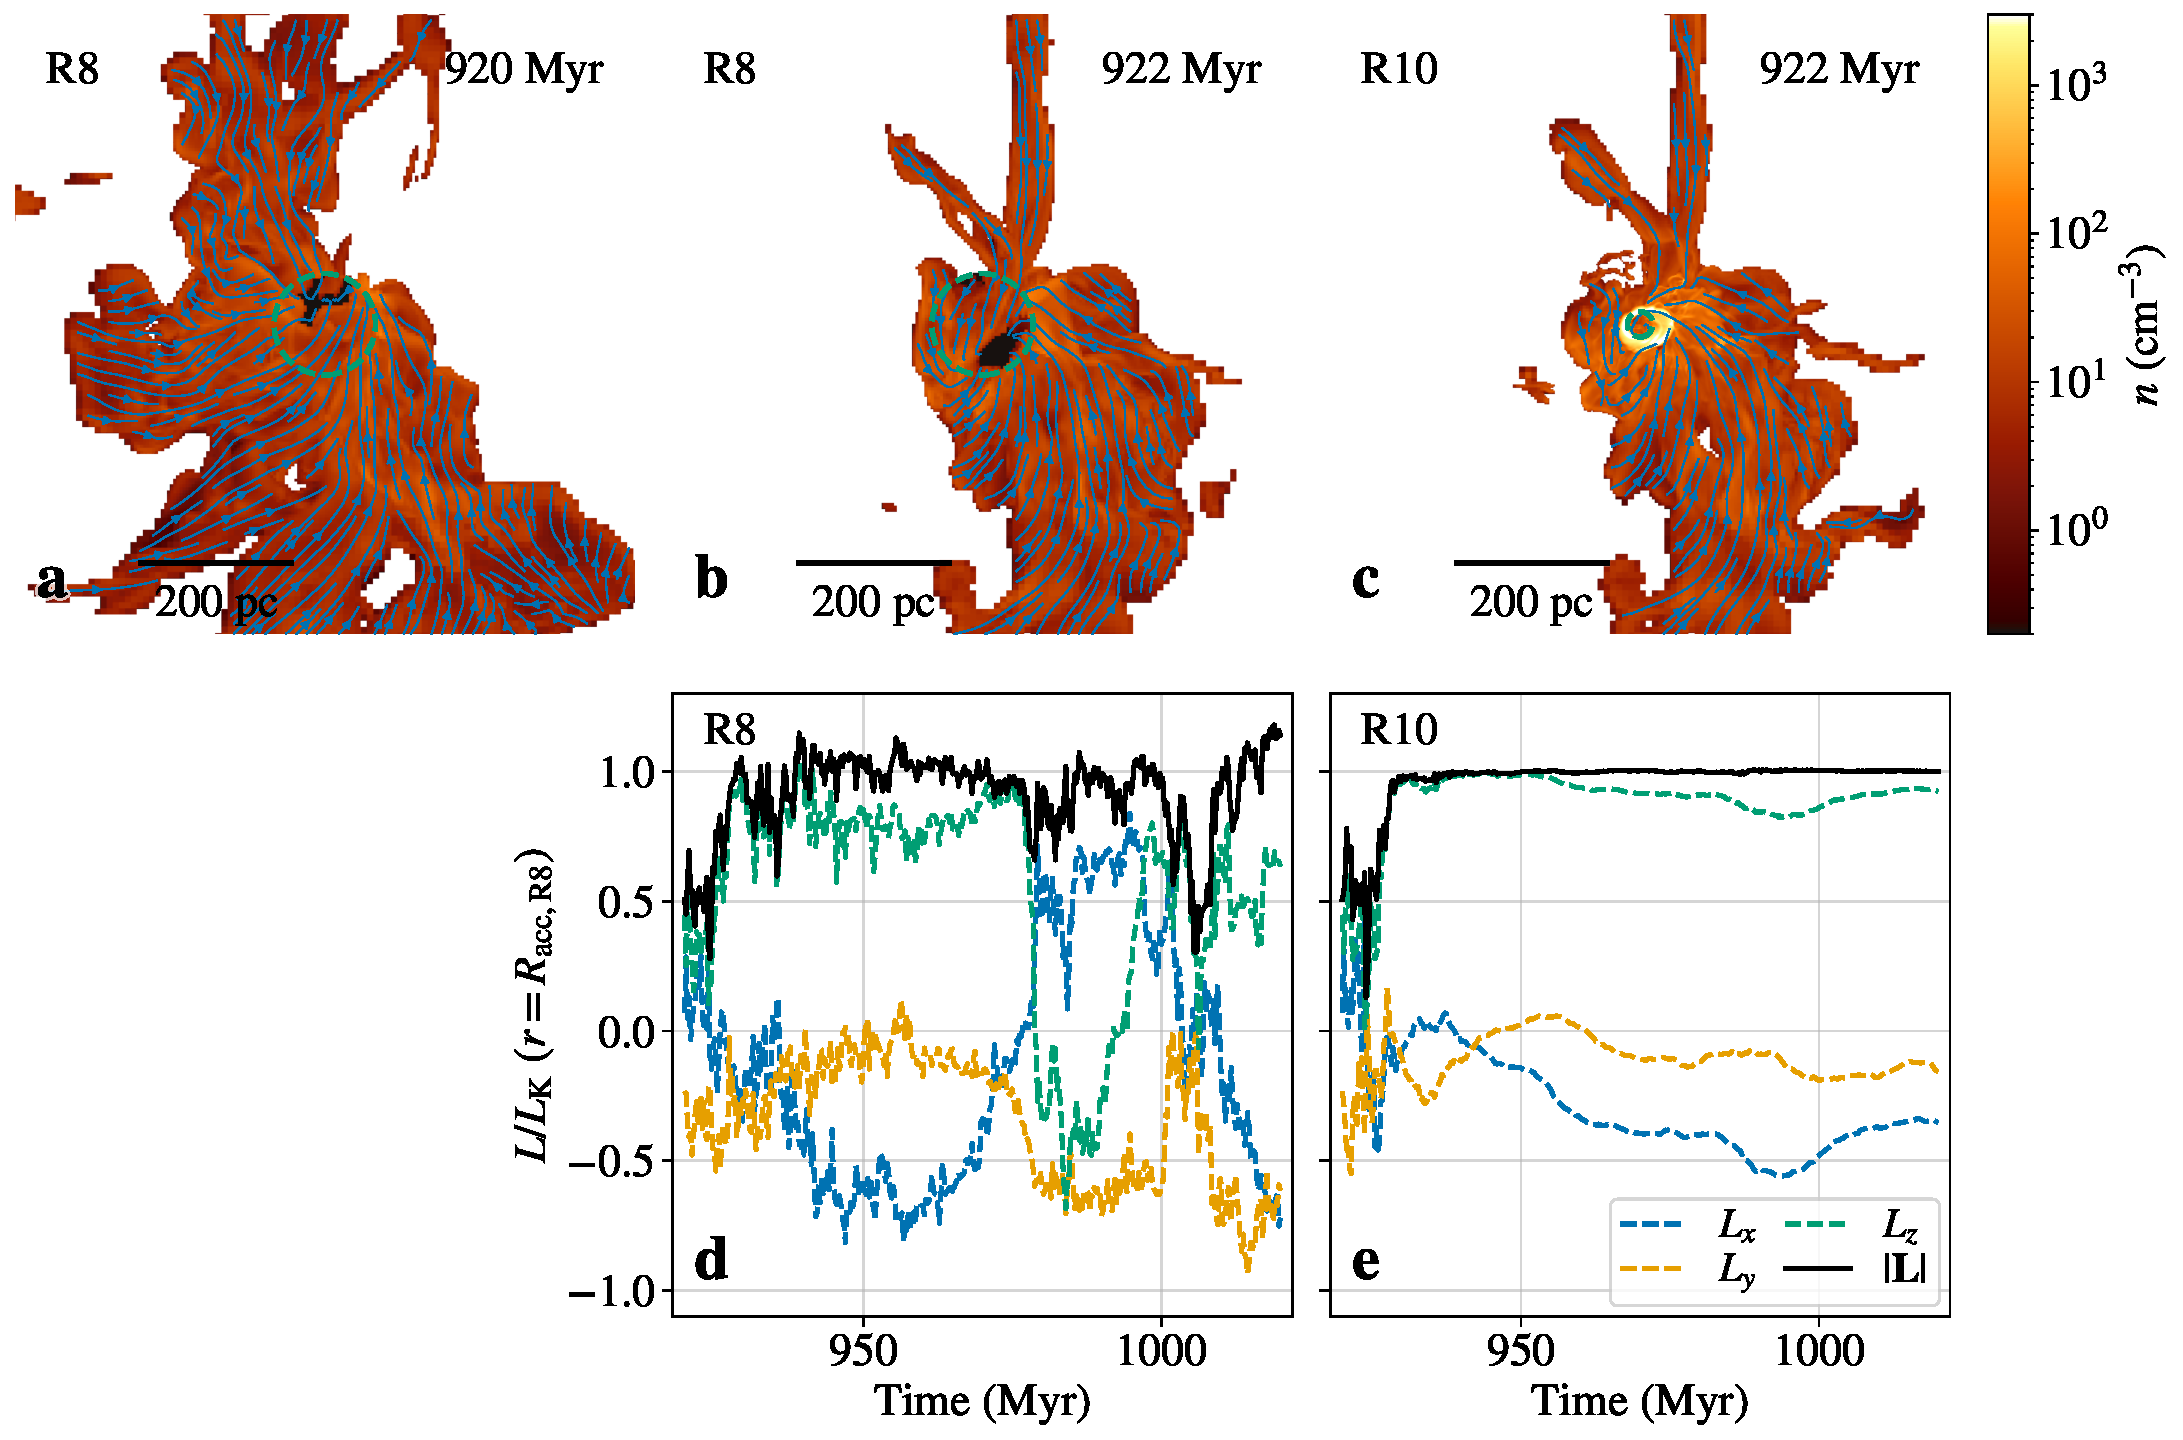
\includegraphics[width=\linewidth]{Sim_img/resolution_exhibit.pdf}
    \caption{
    Top: Projections along the $z$-axis of the number density for the cool gas ($T < 10^6\,K$), with streamlines showing the projected velocity field. Panel (a) shows the fiducial R8 simulation at $t=920\,{\rm Myr}$. Panels (b) and (c) show the evolved morphology at $t=922\,{\rm Myr}$ for the R8 and R10 simulations, respectively. The green dashed circles mark their respective accretion zones. Bottom: normalized specific angular momentum, measured at the same physical radius, $r=R_{\rm acc,R8}\approx65\,{\rm pc}$, for the R8 and R10 runs, recorded over a 100\,Myr evolution. The colored dashed curves show $L_x$, $L_y$, and $L_z$, while the black solid curve shows $|\mathbf{L}|$.
    \label{fig:resolution-exhibit}}
\end{figure}

\subsubsection{Limitations and future work}
\label{subsec:limitations}

The simulations we presented in this work probe gas dynamics across eight orders of magnitude in spatial scale
and nine orders of magnitude in time.
To achieve this vast scale separation, we omit several physical processes which we do not expect to have a significant impact on the overall gas distribution.
Here, we discuss the potential effects of these neglected processes.

Our simulations are purely hydrodynamic and neglect the effects of magnetic fields.
In galaxy clusters, the ICM is weakly magnetized, with plasma $\beta \sim 10^2$--$10^3$ (the ratio between thermal pressure and magnetic pressure).
In the hot phase, \citet{guo_magnetized_2024} found that magnetic energy becomes dynamically important around $r \sim 10^4$\,\rg.
In the cool phase, $\beta \sim 1$\ even at scales $\gtrsim 10^5$\,\rg. Magnetic fields appear to enhance angular momentum loss in the cool phase, which could shrink the disk by a factor of $\sim 10$\ \citep[e.g.,][]{wang_chaotic_2020}.
In the meso-scale simulation, our cool disk extends to $R_{\rm disk}\approx600$\,pc; a $10\times$\ smaller disk would appear consistent with \textit{HST} observations of a circumnuclear disk at the 40\,pc scale \citep[][]{walsh_m87_2013}.
We expect the qualitative results of a galaxy-scale MHD simulation to be similar to the hydrodynamic case, but the radial extent of the cool gas might differ.
At the meso-scale, magnetic flux advected by the large-scale accretion flow dictates the field geometry of the accretion disk \citep[][]{lubow_magnetic_1994}.
Jet production also depends on the magnetic pressure within the accretion flow \citep[e.g.,][]{proga_magnetohydrodynamic_2005}.

Our simulations employ a relatively high temperature floor, $T_{\rm floor} = 2\times 10^5$\,K.
We use this temperature floor for two reasons: (1) a lower temperature floor results in more restrictive time steps, and (2) the current resolution is insufficient to resolve the scale height of the cool disk at lower temperatures.
We run the R14 simulation at $t\approx1460$\,Myr with $T_{\rm floor} = 10^4$\,K for $\Delta t= 2\,$Myr, and find that the overall gas distribution remains consistent with the fiducial runs, but the disk quickly loses thermal pressure support and collapses vertically such that the large-scale disk becomes a thin disk ($H/R < 0.1$).
Similar behavior was seen in earlier studies \citep[e.g.,][]{guo_toward_2023}.

We do not track star formation in our simulations. The star formation rate in M87 is several orders of magnitude lower than the black hole accretion rate, $\sim 10^{-5}$--$10^{-3}\,\mathrm{M_{\odot}\,yr^{-1}}$ \citep[e.g.,][]{tan_star-forming_2005,tamhane_constraining_2025}, thanks to efficient star-formation quenching by AGN feedback.
Supernova (SN) feedback and stellar winds from AGB stars are also neglected.
These processes would inject energy into the ISM, but would not meaningfully alter the ICM gas dynamics, since jet feedback is the dominant mode of heating at large scales.
At the pc and sub-pc scales, however, Type Ia SNe have been shown to provide significant local heating in the ISM \citep[][]{li_impact_2020}.
Future work will explore how SN feedback in the circumnuclear disk affects the galaxy's turbulent dynamics.

As discussed in \fullsectionref{subsec:meso}, jet feedback is turned off in the R16, R18, and R20 meso-scale simulations.
With magnetic fields, the jet would emerge self-consistently at the meso-scale, ensuring that heating is continuous as we zoom in to the center, as demonstrated by \citet{guo_magnetized_2024}.


\subsection{Conclusions} \label{sec:conclusion}

We introduce a suite of simulations of a radio-mode elliptical galaxy, using initial conditions informed by \textit{Chandra} observations of M87 and the Virgo cluster.
We model the multi-scale, multiphase accretion onto M87 by implementing a hyper-refinement scheme, progressively adding more nested refinement levels to the center of lower-resolution simulations.
This scheme allows us to study the multiphase gas formation at the $\sim$\,kpc scale facilitated by AGN-jet-driven turbulence, then follow the accretion flow down through the meso-scale to just beyond the event-horizon-scale ($r\sim 100$\,\rg).

In this paper, we introduce our simulations, present a study of the overall multiphase dynamics, and examine the inflow-outflow solution at different length- and time-scales.
Our simulations recover the filamentary cool gas formation at the $\sim$\,kpc scale, induced by interactions between the jet and the galaxy (see Figures~\ref{fig:thermodynamics} and~\ref{fig:resolution-exhibit}).

The cool gas filaments carry angular momentum and circularize into a disk around the inner boundary of the simulation (Figures~\ref{fig:zoom-in-proj} and~\ref{fig:l-m-dot-meso}).
Outside $10^3$\,\rg, the motions of the hot and cool phases are completely decoupled. The cool gas exists primarily in Keplerian disks; the hot gas moves more radially. Inside $10^3$\,\rg, the cool gas is compression-heated to higher temperatures and results in a hot accretion disk at the smallest scale probed by our meso-scale simulation (top panel of Figure~\ref{fig:l-m-dot-meso}).

At the galaxy-scale, cool gas accretion dominates over hot gas accretion, often by a factor of $10$\ or more.
This behavior holds true throughout the length scales, down to $\sim 200$\,\rg\ where the cool gas is heated to much higher temperatures, leaving only the hot phase to be accreted through the smallest accretion zone ($R_{\rm acc,R20} \approx 50$\,\rg). The accretion rate is weakly variable in M87 at this scale. The accretion rate at the inner boundary only fluctuates by a factor of $\sim 2$\ over 1\,kyr. In the three high-resolution runs we perform, the profiles of the net inflow rate all follow power-law scalings, $\dot{M} \propto r^k$, where $0.40 \leq k \leq 0.69$. These results broadly agree with previous RIAF simulations that motivate our adopted accretion-rate calibration.

The Bondi model predicts the hot gas net inflow rate, but not the cool gas flow or the \mrrelation\ scaling. We propose estimating \mdotbh\ from the hot gas beyond the cool-gas precipitation radius ($r\gtrsim 2$\,kpc).

Our galaxy-scale simulation shows periods of chaotic, filamentary cool gas accretion, followed by brief disky phases in the first half of its 2\,Gyr evolution. The large-scale disk ($R_{\rm disk}\sim 0.5$--$1$\,kpc) takes over the late-stage evolution. Further examination, however, points toward a constant presence of the disky phase regardless of whether kpc-scale cool filaments are present. We suggest that previous simulations either did not have enough resolution to resolve the circumnuclear disk ($R_{\rm disk}\sim 10$--$100$\,pc), or the accretion boundary was too large to allow cool gas to circularize and form a disk.
